% 図解レジュメ: the method of the 26f WIP resume (OLR) explained one step per figure.  Same notation and numbers as the resume (ol7):
%   numbers_ol.tex is copied from it; CIFAR-10 values (p = 23, 34 blocks, block A = the 23rd, Delta = 1.768, n = 2,000) are from the
%   resume's gen/data/ol (olx_info.json, hl_meta.json).  The clouds, the channel map and the curves of Figure 3(b) are schematic
%   (gen/mk_data.py).  Notation: scalars plain, vectors with arrows (p x 1 columns), matrices bold.
% Layout: one column (class option onecolumn); every figure and table is placed with [H] right where its step is explained.
% build: python3 gen/mk_data.py && latexmk -r latexmkrc main.tex
\documentclass[MIRU,submit,onecolumn]{miru2025j}
\usepackage[dvipdfmx]{graphicx}
\usepackage[dvipdfmx]{xcolor}
\definecolor{navyc}{RGB}{31,58,122}\definecolor{redc}{RGB}{192,57,43}
\usepackage{amsmath,amssymb}
\usepackage{booktabs}
\usepackage{array}
\usepackage{float}   % [H]: each figure stays where its step is explained
\usepackage{tikz}
\usetikzlibrary{arrows.meta,calc,decorations.pathreplacing}
\newcommand{\Ours}{OLR}
\newcommand{\cn}[1]{\tikz[baseline=(cn.base)]\node[circle, draw, line width=0.4pt, inner sep=0.6pt, font=\scriptsize](cn){#1};}   % circled step numbers (U+2460.. are not in pLaTeX)
\newcommand{\vmu}{\vec{\mu}}\newcommand{\va}{\vec{a}}\newcommand{\vx}{\vec{x}}\newcommand{\vu}{\vec{u}}\newcommand{\vv}{\vec{v}}
\newcommand{\Pm}{\mathbf{P}}\newcommand{\Sm}{\mathbf{S}}\newcommand{\Id}{\mathbf{I}}\newcommand{\Gm}{\mathbf{G}}
% written by gen/ol_gen.py
\newcommand{\olTestOL}{95.6}
\newcommand{\olTestVf}{84.7}
\newcommand{\olSixMin}{95.3}
\newcommand{\olSixMax}{95.7}
\newcommand{\olSixMean}{95.5}
\newcommand{\olSixMeanB}{95.51}
\newcommand{\olSixVf}{84.8}
\newcommand{\olSixVfMin}{84.3}
\newcommand{\olSixVfMax}{85.1}
\newcommand{\olSixHf}{58.5}
\newcommand{\olSixFpr}{17.9}
\newcommand{\olSixAll}{95.4}
\newcommand{\olSixL}{94.4}
\newcommand{\olSixT}{87.5}
\newcommand{\olSixAllGap}{0.12}
\newcommand{\olSixLGap}{1.1}
\newcommand{\olSixTGap}{8.0}
\newcommand{\olSixCten}{95.1}
\newcommand{\olSixAllCten}{93.4}
\newcommand{\olSixLCten}{94.9}
\newcommand{\olSixTCten}{76.3}
\newcommand{\olSixVfCten}{88.4}
\newcommand{\olSixHfCten}{50.2}
\newcommand{\olSixMinCten}{94.2}
\newcommand{\olSixMaxCten}{95.8}
\newcommand{\olSixSVHN}{96.9}
\newcommand{\olSixAllSVHN}{99.5}
\newcommand{\olSixLSVHN}{95.2}
\newcommand{\olSixTSVHN}{90.6}
\newcommand{\olSixVfSVHN}{63.9}
\newcommand{\olSixHfSVHN}{68.2}
\newcommand{\olSixMinSVHN}{96.6}
\newcommand{\olSixMaxSVHN}{97.1}
\newcommand{\olSixCelebA}{100.0}
\newcommand{\olSixAllCelebA}{100.0}
\newcommand{\olSixLCelebA}{100.0}
\newcommand{\olSixTCelebA}{100.0}
\newcommand{\olSixVfCelebA}{99.9}
\newcommand{\olSixHfCelebA}{50.0}
\newcommand{\olSixMinCelebA}{99.9}
\newcommand{\olSixMaxCelebA}{100.0}
\newcommand{\olSixIN}{85.9}
\newcommand{\olSixAllIN}{84.3}
\newcommand{\olSixLIN}{82.3}
\newcommand{\olSixTIN}{73.1}
\newcommand{\olSixVfIN}{74.7}
\newcommand{\olSixHfIN}{50.2}
\newcommand{\olSixMinIN}{84.6}
\newcommand{\olSixMaxIN}{87.1}
\newcommand{\olSixFM}{99.7}
\newcommand{\olSixAllFM}{99.7}
\newcommand{\olSixLFM}{99.6}
\newcommand{\olSixTFM}{97.6}
\newcommand{\olSixVfFM}{97.1}
\newcommand{\olSixHfFM}{74.0}
\newcommand{\olSixMinFM}{99.4}
\newcommand{\olSixMaxFM}{99.8}
\newcommand{\olEqSix}{91.9}
\newcommand{\olEqSixMin}{91.6}
\newcommand{\olEqSixMax}{92.1}
\newcommand{\olEqSixDrop}{3.6}
\newcommand{\olEqSixVf}{80.6}
\newcommand{\olEqSixCten}{88.7}
\newcommand{\olEqSixDropCten}{6.4}
\newcommand{\olEqSixSVHN}{97.1}
\newcommand{\olEqSixDropSVHN}{-0.3}
\newcommand{\olEqSixCelebA}{100.0}
\newcommand{\olEqSixDropCelebA}{0.0}
\newcommand{\olEqSixIN}{74.7}
\newcommand{\olEqSixDropIN}{11.3}
\newcommand{\olEqSixFM}{99.0}
\newcommand{\olEqSixDropFM}{0.7}
\newcommand{\olNCten}{258}
\newcommand{\olNTex}{199}
\newcommand{\olNBlkCten}{23}
\newcommand{\olNRefMin}{1{,}500}
\newcommand{\olNRefMax}{2{,}000}
\newcommand{\olNStored}{552}
\newcommand{\olMBOurs}{0.0011}
\newcommand{\olDeltaMin}{0.9}
\newcommand{\olDeltaMax}{8.8}
\newcommand{\olNBlkMin}{8}
\newcommand{\olNBlkMax}{25}
\newcommand{\olDeltaCten}{1.8}
\newcommand{\olDeltaSVHN}{1.1}
\newcommand{\olDeltaCelebA}{8.8}
\newcommand{\olDeltaIN}{0.9}
\newcommand{\olDeltaFM}{2.8}
\newcommand{\olHrNCal}{1{,}000}
\newcommand{\olHrNBlk}{22}
\newcommand{\olSecOL}{0.068}
\newcommand{\olFwdAll}{0.180}
\newcommand{\olFwdA}{0.066}
\newcommand{\olFwdAShare}{37}
\newcommand{\olJudgeMs}{1.8}
\newcommand{\olSecCfs}{0.181}
\newcommand{\olSecCfsStop}{0.087}
\newcommand{\olSecCfsKnn}{0.185}
\newcommand{\olSecCfsKnnStop}{0.090}
\newcommand{\olSecRatioCfsKnn}{0.75}
\newcommand{\olSecRatioCfs}{0.79}
\newcommand{\olSecRatioCfsKnnFull}{0.37}
\newcommand{\olCpuHere}{Intel Core i9-7920X, 2.90\,GHz}
\newcommand{\olPairs}{51}
\newcommand{\olNPrior}{10}
\newcommand{\olNStat}{8}
\newcommand{\olBestPriorName}{CFSの kNN ヘッド}
\newcommand{\olBestPriorMean}{88.0}
\newcommand{\olGapCfsKnn}{7.6}
\newcommand{\olGapCfsKnnLo}{7.0}
\newcommand{\olGapCfsKnnHi}{8.3}
\newcommand{\olGapCfs}{10.0}
\newcommand{\olGapCfsLo}{9.3}
\newcommand{\olGapCfsHi}{10.7}
\newcommand{\olCfsMean}{85.6}
\newcommand{\olVfBestPriorName}{EigenScore}
\newcommand{\olVfBestPriorAvg}{78.6}
\newcommand{\olPriorBestCten}{85.4}
\newcommand{\olPriorBestCtenName}{CFSの kNN ヘッド}
\newcommand{\olTestCten}{95.6}
\newcommand{\olPriorBestGapCten}{$+$10.2}
\newcommand{\olGapCfsKnnCten}{$+$10.2}
\newcommand{\olVerdictCfsKnnCten}{win}
\newcommand{\olPriorBestSVHN}{99.8}
\newcommand{\olPriorBestSVHNName}{DiffPath}
\newcommand{\olTestSVHN}{96.9}
\newcommand{\olPriorBestGapSVHN}{$-$2.9}
\newcommand{\olGapCfsKnnSVHN}{$+$3.2}
\newcommand{\olVerdictCfsKnnSVHN}{win}
\newcommand{\olPriorBestCelebA}{99.8}
\newcommand{\olPriorBestCelebAName}{DiffPath}
\newcommand{\olTestCelebA}{100.0}
\newcommand{\olPriorBestGapCelebA}{$+$0.2}
\newcommand{\olGapCfsKnnCelebA}{$+$0.4}
\newcommand{\olVerdictCfsKnnCelebA}{win}
\newcommand{\olPriorBestIN}{65.5}
\newcommand{\olPriorBestINName}{CFS}
\newcommand{\olTestIN}{85.8}
\newcommand{\olPriorBestGapIN}{$+$20.3}
\newcommand{\olGapCfsKnnIN}{$+$24.4}
\newcommand{\olVerdictCfsKnnIN}{win}
\newcommand{\olPriorBestFM}{99.8}
\newcommand{\olPriorBestFMName}{CFSの kNN ヘッド}
\newcommand{\olTestFM}{99.8}
\newcommand{\olPriorBestGapFM}{$+$0.0}
\newcommand{\olGapCfsKnnFM}{$+$0.0}
\newcommand{\olVerdictCfsKnnFM}{tie}
\newcommand{\olPriorWinMin}{34}
\newcommand{\olPriorWinMax}{50}
\newcommand{\olWtlCfsKnn}{37/14/0}
\newcommand{\olWtlCfs}{42/9/0}
\newcommand{\olPriorLossMax}{10}
\newcommand{\olPriorLossMaxName}{MSMA型, DiffPath}
\newcommand{\olNLostPrior}{11}
\newcommand{\olNLostPriorSVHN}{11}
\newcommand{\olNLostPriorVf}{1}
\newcommand{\olLostPriorList}{SVHNの上下反転(EigenScore), SVHNを分布内とするCIFAR-10(NLL・TT・MSMA型・DiffPath), SVHNを分布内とするCIFAR-100(NLL・TT・MSMA型・DiffPath), SVHNを分布内とするCelebA(NLL・TT・MSMA型・DiffPath), SVHNを分布内とするTextures(MSMA型・DiffPath), SVHNを分布内とするTiny-ImageNet(NLL・TT・MSMA型・DiffPath), SVHNを分布内とするLSUN(NLL・IC-PNG・TT・MSMA型・DiffPath), SVHNを分布内とするImageNet(NLL・TT・MSMA型・DiffPath), SVHNを分布内とするImageNet32(NLL・IC-PNG・TT・MSMA型・DiffPath), SVHNを分布内とするPlaces365(NLL・TT・MSMA型・DiffPath), SVHNを分布内とする一様ノイズ(NLL・IC-PNG・IC-J2K・TT・MSMA型・DiffPath)}
\newcommand{\olOursColsBest}{6}
\newcommand{\olUnderlineNote}{}
\newcommand{\olTestSVHNBehind}{2.9}
\newcommand{\olTestFMBehind}{0.0}
\newcommand{\olNImgCfs}{50{,}000}
\newcommand{\olMBCfsKnn}{102}
\newcommand{\olImgRatio}{25}
\newcommand{\olEqOL}{92.0}
\newcommand{\olEqCfs}{82.5}
\newcommand{\olEqCfsKnn}{84.4}
\newcommand{\olOrigCfs}{85.6}
\newcommand{\olOrigCfsKnn}{88.0}
\newcommand{\olEqDropOL}{3.6}
\newcommand{\olEqDropCfs}{3.2}
\newcommand{\olEqDropCfsKnn}{3.6}
\newcommand{\olEqGapCfsKnn}{7.6}
\newcommand{\olEqGapCfsKnnLo}{6.9}
\newcommand{\olEqGapCfsKnnHi}{8.4}
\newcommand{\olEqGapCfs}{9.6}
\newcommand{\olEqGapCfsLo}{8.7}
\newcommand{\olEqGapCfsHi}{10.4}
\newcommand{\olOrigGapCfsKnnB}{7.6}
\newcommand{\olOrigGapCfsKnnBLo}{7.0}
\newcommand{\olOrigGapCfsKnnBHi}{8.3}
\newcommand{\olEqWtlCfsKnn}{36/3/4}
\newcommand{\olEqWtlCfs}{43/0/0}
\newcommand{\olEqNPairs}{43}
\newcommand{\olOrigWtlCfsKnnB}{35/8/0}
\newcommand{\olEqNLostCfsKnn}{4}
\newcommand{\olEqLostCfsKnnList}{FashionMNISTを分布内とするMNIST, FashionMNISTを分布内とするKMNIST, FashionMNISTを分布内とするOmniglot, FashionMNISTを分布内とするnotMNIST}
\newcommand{\olEqGapCfsKnnCten}{$+$13.5}
\newcommand{\olEqOLCten}{88.9}
\newcommand{\olEqCfsKnnCten}{75.4}
\newcommand{\olEqGapCfsKnnSVHN}{$+$3.6}
\newcommand{\olEqOLSVHN}{97.3}
\newcommand{\olEqCfsKnnSVHN}{93.6}
\newcommand{\olEqGapCfsKnnCelebA}{$+$0.3}
\newcommand{\olEqOLCelebA}{100.0}
\newcommand{\olEqCfsKnnCelebA}{99.7}
\newcommand{\olEqGapCfsKnnIN}{$+$21.6}
\newcommand{\olEqOLIN}{75.0}
\newcommand{\olEqCfsKnnIN}{53.4}
\newcommand{\olEqGapCfsKnnFM}{$-$1.0}
\newcommand{\olEqOLFM}{98.9}
\newcommand{\olEqCfsKnnFM}{99.9}
\newcommand{\olTestFpr}{18.6}
\newcommand{\olCfsKnnFpr}{35.9}
\newcommand{\olCfsFpr}{45.5}
\newcommand{\olEqVfOL}{80.3}
\newcommand{\olEqVfCfsKnn}{72.3}
\newcommand{\olCfsValMean}{86.8}
\newcommand{\olCfsKnnValMean}{88.1}
\newcommand{\olGapCfsKnnVal}{7.6}
\newcommand{\olDqOLMin}{62.7}
\newcommand{\olDqOLMax}{90.0}
\newcommand{\olDqOLMean}{76.5}
\newcommand{\olDqCfsKnnMin}{64.0}
\newcommand{\olDqCfsKnnMax}{88.7}
\newcommand{\olDqCfsKnnMean}{74.5}
\newcommand{\olDqCfsMin}{57.4}
\newcommand{\olDqCfsMax}{88.9}
\newcommand{\olDqCfsMean}{72.8}
\newcommand{\olDqLMin}{58.7}
\newcommand{\olDqLMax}{81.4}
\newcommand{\olDqLMean}{70.1}
\newcommand{\olDqTMin}{66.2}
\newcommand{\olDqTMax}{91.6}
\newcommand{\olDqTMean}{78.4}
\newcommand{\olDqNHigher}{5}
\newcommand{\olDqSVHNMax}{66.5}
\newcommand{\olDqINJpeg}{98.5}
\newcommand{\olDqCfsKnnINJpeg}{71.0}
\newcommand{\olDqBlurOL}{90.0}
\newcommand{\olDqBlurCfsKnn}{88.7}
\newcommand{\olDqBlurHalfOL}{62.7}
\newcommand{\olDqJpegOL}{69.0}
\newcommand{\olDqJpegCfsKnn}{64.7}
\newcommand{\olVarTrained}{95.5}
\newcommand{\olVarRinit}{72.0}
\newcommand{\olVarRshuf}{67.9}
\newcommand{\olVarRinitVf}{55.3}
\newcommand{\olVarRshufVf}{56.9}
\newcommand{\olVarTrainedVf}{85.0}
\newcommand{\olVarBy}{84.2}
\newcommand{\olVarByTrained}{97.0}
\newcommand{\olVarByL}{64.1}
\newcommand{\olVarByT}{84.9}
\newcommand{\olVarByVf}{59.4}
\newcommand{\olVarNBy}{6}
\newcommand{\olVarByMin}{60.0}
\newcommand{\olVarByMax}{99.4}
\newcommand{\olVarRinitL}{57.9}
\newcommand{\olVarRinitT}{73.1}
\newcommand{\olVarTrainedL}{94.5}
\newcommand{\olVarTrainedT}{87.3}
\newcommand{\olVarRinitCten}{65.4}
\newcommand{\olVarRshufCten}{62.3}
\newcommand{\olVarRinitSVHN}{74.8}
\newcommand{\olVarRshufSVHN}{70.7}
\newcommand{\olVarRinitCelebA}{77.0}
\newcommand{\olVarRshufCelebA}{76.4}
\newcommand{\olVarRinitIN}{60.7}
\newcommand{\olVarRshufIN}{60.2}
\newcommand{\olVarRinitFM}{81.8}
\newcommand{\olVarRshufFM}{69.9}
\newcommand{\olDevCzero}{87.8}
\newcommand{\olDevEqCzero}{83.2}
\newcommand{\olDevCone}{91.9}
\newcommand{\olDevEqCone}{86.8}
\newcommand{\olDevCfour}{94.9}
\newcommand{\olDevEqCfour}{90.6}
\newcommand{\olDevCeight}{95.6}
\newcommand{\olDevEqCeight}{91.8}
\newcommand{\olDevCsixteen}{95.6}
\newcommand{\olDevEqCsixteen}{92.0}
\newcommand{\olDevCsixtyfour}{95.0}
\newcommand{\olDevEqCsixtyfour}{91.0}
\newcommand{\olDevCinf}{94.5}
\newcommand{\olDevEqCinf}{90.1}
\newcommand{\olDevOv}{95.3}
\newcommand{\olDevEqOv}{91.3}
\newcommand{\olDevOnomirror}{95.6}
\newcommand{\olDevEqOnomirror}{91.9}
\newcommand{\olDevOquarter}{95.5}
\newcommand{\olDevEqOquarter}{91.6}
\newcommand{\olDevOflips}{95.0}
\newcommand{\olDevEqOflips}{90.9}
\newcommand{\olDevNfifty}{93.3}
\newcommand{\olDevEqNfifty}{88.4}
\newcommand{\olDevNhundred}{93.8}
\newcommand{\olDevEqNhundred}{89.7}
\newcommand{\olDevNfivehundred}{94.9}
\newcommand{\olDevEqNfivehundred}{90.8}
\newcommand{\olDevNthousand}{95.6}
\newcommand{\olDevEqNthousand}{91.5}
\newcommand{\olDevAll}{95.3}
\newcommand{\olDevEqAll}{90.9}
\newcommand{\olDevLstd}{95.2}
\newcommand{\olDevEqLstd}{91.2}
\newcommand{\olDevPk}{94.5}
\newcommand{\olDevEqPk}{90.2}
\newcommand{\olDevPkd}{91.2}
\newcommand{\olDevEqPkd}{86.1}
\newcommand{\olDevPkds}{91.2}
\newcommand{\olDevEqPkds}{85.7}
\newcommand{\olDevVfCeight}{85.2}
\newcommand{\olDevVfCinf}{87.0}
\newcommand{\olDevVfPk}{87.2}
\newcommand{\olDevSVHNOv}{96.0}
\newcommand{\olDevSVHNOquarter}{97.3}
\newcommand{\olDevCeightB}{95.55}
\newcommand{\olDevEqCeightB}{91.77}
\newcommand{\olDevSVHNAll}{99.5}
\newcommand{\olDevSVHNCeight}{97.3}
\newcommand{\olNVar}{35}
\newcommand{\olVarSixName}{全ブロック, $c=16$}
\newcommand{\olVarSixNat}{95.47}
\newcommand{\olVarSixEq}{90.61}
\newcommand{\olVarSevenEq}{91.76}
\newcommand{\olVarEightNat}{95.59}
\newcommand{\olVarEightEq}{91.68}
\newcommand{\olCandEightNat}{95.54}
\newcommand{\olCandEightEq}{91.66}
\newcommand{\olCandSevenBest}{94.67}
\newcommand{\olCandSevenBestEq}{90.74}
\newcommand{\olNDev}{62}
\newcommand{\olDevSeeds}{95.54, 95.55, 95.56}
\newcommand{\olDevSeedsEq}{91.66, 91.88, 91.78}
\newcommand{\olDevCutMin}{83}
\newcommand{\olDevCutMax}{85}
\newcommand{\olOracleCosMin}{0.72}
\newcommand{\olOracleCosMax}{0.86}
\newcommand{\olCosMin}{0.71}
\newcommand{\olCosMax}{0.87}
\newcommand{\olBarNat}{95.07}
\newcommand{\olBarEq}{90.33}
\newcommand{\olDevDiff}{0.003}
\newcommand{\olFallOrMin}{38}
\newcommand{\olFallOrMax}{65}
\newcommand{\olRiseOrMax}{21}
\newcommand{\olZaOrMin}{-7.6}
\newcommand{\olZaOrMax}{-0.6}
\newcommand{\olFallOodMin}{26}
\newcommand{\olFallOodMax}{81}
\newcommand{\olRiseOodSVHN}{55}
\newcommand{\olFallOodSVHN}{26}
\newcommand{\olNSetsA}{38}
\newcommand{\olNSetsAMargin}{36}
\newcommand{\olIdZaAbsMax}{0.08}
\newcommand{\olSignIdMin}{0}
\newcommand{\olSignIdMax}{94}
\newcommand{\olKapMin}{0.83}
\newcommand{\olKapMax}{1.65}
\newcommand{\olKapNLeOne}{4}
\newcommand{\olKapCelebA}{1.65}
\newcommand{\olKapWMin}{0.82}
\newcommand{\olKapWMax}{0.95}
\newcommand{\olKapIdMin}{0.95}
\newcommand{\olKapIdMax}{1.00}
\newcommand{\olXOLR}{95.6}
\newcommand{\olXDir}{94.5}
\newcommand{\olXPool}{97.0}
\newcommand{\olXSet}{98.1}
\newcommand{\olXSsbSet}{81.1}
\newcommand{\olXSsbOLR}{64.3}
\newcommand{\olXCHundredSet}{91.3}
\newcommand{\olXCHundredOLR}{89.8}
\newcommand{\olDevMGeight}{95.61}
\newcommand{\olHrOL}{76.3}
\newcommand{\olHrOLNear}{70.8}
\newcommand{\olHrOLFar}{80.0}
\newcommand{\olHrOLVf}{60.4}
\newcommand{\olHrCfs}{73.4}
\newcommand{\olHrCfsNear}{68.0}
\newcommand{\olHrCfsFar}{77.0}
\newcommand{\olHrCfsVf}{49.3}
\newcommand{\olHrCfsKnn}{66.2}
\newcommand{\olHrCfsKnnNear}{68.5}
\newcommand{\olHrCfsKnnFar}{64.6}
\newcommand{\olHrCfsKnnVf}{50.5}
\newcommand{\olHrL}{60.3}
\newcommand{\olHrLNear}{51.9}
\newcommand{\olHrLFar}{65.9}
\newcommand{\olHrLVf}{68.4}
\newcommand{\olHrT}{76.4}
\newcommand{\olHrTNear}{74.2}
\newcommand{\olHrTFar}{77.9}
\newcommand{\olHrTVf}{48.1}
\newcommand{\olHrAll}{82.7}
\newcommand{\olHrAllNear}{81.0}
\newcommand{\olHrAllFar}{83.8}
\newcommand{\olHrAllVf}{65.1}
\newcommand{\olHrGapCfs}{$+$2.9}
\newcommand{\olHrGapCfsLo}{$+$1.3}
\newcommand{\olHrGapCfsHi}{$+$4.4}
\newcommand{\olHrWtlCfs}{4/0/2}
\newcommand{\olHrGapCfsKnn}{$+$10.1}
\newcommand{\olHrGapCfsKnnLo}{$+$8.2}
\newcommand{\olHrGapCfsKnnHi}{$+$12.0}
\newcommand{\olHrWtlCfsKnn}{5/0/1}
\newcommand{\olHrOLSsb}{64.6}
\newcommand{\olHrCfsKnnSsb}{69.4}
\newcommand{\olHrCfsSsb}{69.9}
\newcommand{\olHrOLNinco}{77.1}
\newcommand{\olHrCfsKnnNinco}{67.7}
\newcommand{\olHrCfsNinco}{66.1}
\newcommand{\olHrOLInat}{74.5}
\newcommand{\olHrCfsKnnInat}{54.2}
\newcommand{\olHrCfsInat}{60.5}
\newcommand{\olHrOLTex}{94.5}
\newcommand{\olHrCfsKnnTex}{85.6}
\newcommand{\olHrCfsTex}{89.8}
\newcommand{\olHrOLOio}{70.8}
\newcommand{\olHrCfsKnnOio}{54.1}
\newcommand{\olHrCfsOio}{80.6}
\newcommand{\olHrHf}{50.1}
\newcommand{\olHrBestName}{CFS}
\newcommand{\olHdOL}{78.9}
\newcommand{\olHdOLNear}{74.8}
\newcommand{\olHdOLFar}{81.7}
\newcommand{\olHdOLVf}{59.6}
\newcommand{\olHdCfs}{71.0}
\newcommand{\olHdCfsNear}{67.1}
\newcommand{\olHdCfsFar}{73.7}
\newcommand{\olHdCfsVf}{49.4}
\newcommand{\olHdCfsKnn}{63.4}
\newcommand{\olHdCfsKnnNear}{63.3}
\newcommand{\olHdCfsKnnFar}{63.4}
\newcommand{\olHdCfsKnnVf}{50.4}
\newcommand{\olHdL}{67.7}
\newcommand{\olHdLNear}{63.4}
\newcommand{\olHdLFar}{70.6}
\newcommand{\olHdLVf}{65.2}
\newcommand{\olHdT}{75.5}
\newcommand{\olHdTNear}{72.6}
\newcommand{\olHdTFar}{77.4}
\newcommand{\olHdTVf}{47.4}
\newcommand{\olHdAll}{79.4}
\newcommand{\olHdAllNear}{79.8}
\newcommand{\olHdAllFar}{79.1}
\newcommand{\olHdAllVf}{61.6}
\newcommand{\olHdGapCfs}{$+$7.9}
\newcommand{\olHdGapCfsLo}{$+$6.5}
\newcommand{\olHdGapCfsHi}{$+$9.4}
\newcommand{\olHdWtlCfs}{6/0/0}
\newcommand{\olHdGapCfsKnn}{$+$15.6}
\newcommand{\olHdGapCfsKnnLo}{$+$13.7}
\newcommand{\olHdGapCfsKnnHi}{$+$17.4}
\newcommand{\olHdWtlCfsKnn}{6/0/0}
\newcommand{\olHdOLSsb}{80.2}
\newcommand{\olHdCfsKnnSsb}{66.0}
\newcommand{\olHdCfsSsb}{70.5}
\newcommand{\olHdOLNinco}{69.5}
\newcommand{\olHdCfsKnnNinco}{60.7}
\newcommand{\olHdCfsNinco}{63.6}
\newcommand{\olHdOLInat}{72.7}
\newcommand{\olHdCfsKnnInat}{40.8}
\newcommand{\olHdCfsInat}{61.7}
\newcommand{\olHdOLTex}{93.7}
\newcommand{\olHdCfsKnnTex}{84.2}
\newcommand{\olHdCfsTex}{88.7}
\newcommand{\olHdOLOio}{78.6}
\newcommand{\olHdCfsKnnOio}{65.1}
\newcommand{\olHdCfsOio}{70.5}
\newcommand{\olHdHf}{49.4}
\newcommand{\olHdBestName}{CFS}
\newcommand{\olHrFwdA}{3.6}
\newcommand{\olHrFwdAll}{12.1}
\newcommand{\olHrSecCfsStop}{5.3}
\newcommand{\olHrFwdAShare}{30}
\newcommand{\olHrDelta}{0.55}
\newcommand{\olHdDelta}{0.56}
\newcommand{\olHdOLSsbRank}{2}
\newcommand{\olSsbShort}{224}
\newcommand{\olInShort}{375}
\newcommand{\olSsbShare}{94.9}
\newcommand{\olInShare}{10.8}
\newcommand{\olSsbFacts}{99.9}
\newcommand{\olFactsMin}{95.3}

\makeatletter
\renewcommand{\signame}{26f WIP中間発表(手法の図解)}
\renewcommand{\MIRUPreface}{}
\renewenvironment{figure}{\@floatenv\capwidth\textwidth\ecapwidth\textwidth\abovecaptionskip1mm\belowcaptionskip\z@\@float{figure}}{\end@float}
\renewenvironment{table}{\@floatenv\capwidth\textwidth\ecapwidth\textwidth\abovecaptionskip\z@\belowcaptionskip1mm\@float{table}}{\end@float}
\setlength{\@fptop}{0pt}\setlength{\@fpbot}{0pt plus 1fil}
\makeatother
\renewcommand{\eqref}[1]{(\ref{#1})}
\raggedbottom
\begin{document}
\title{\textbf{図解 \Ours{}\\向きを変えた分布内画像による拡散モデルの分布外検知}}
\affiliate{sfc}{慶應義塾大学 総合政策学部B3 中澤・大越研究室 d-hacks}
\affiliate{sfc2}{慶應義塾大学大学院 政策・メディア研究科}
\author{omote}{}{sfc}[]
\author{親:zackeyさん}{}{sfc2}[]
\maketitle

\begin{figure}[H]\centering
% f1_overview.tex -- Figure 1 (in the title block): the three steps of the method in one row (natural width about 17.4 cm).
%   Colours: navy = in-distribution side, grey = re-oriented images, red = what is computed for the test image and the point mu*.
%   Panels 2 and 3 are schematics (the drawing to scale is Figure 4; there mu* is 8 times as far from mu as mu_o).
\begin{tikzpicture}[>={Stealth[length=2mm, width=1.6mm]}, font=\footnotesize, line cap=round, line join=round,
  ttl/.style={anchor=north west, inner sep=0pt, font=\small}, lab/.style={font=\footnotesize, inner sep=1pt, align=center},
  sm/.style={font=\scriptsize, inner sep=1pt, align=center}]
% frames of the three steps (no fill)
\draw[black!40, rounded corners=4pt] (0,0) rectangle (5.5,3.9);
\draw[black!40, rounded corners=4pt] (5.95,0) rectangle (11.45,3.9);
\draw[black!40, rounded corners=4pt] (11.9,0) rectangle (17.4,3.9);
\draw[->, very thick] (5.55,1.9) -- (5.9,1.9);
\draw[->, very thick] (11.5,1.9) -- (11.85,1.9);
% ---------------------------------------------------------------- 1
\node[ttl] at (0.15,3.75) {\textbf{1.}\ 画像1枚から数を $p$ 個とる};
\node[inner sep=0, draw=black!50, line width=0.4pt] (im) at (0.75,1.85) {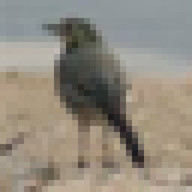
\includegraphics[width=1.05cm]{img/b_o0.png}};
\node[lab, anchor=north] at (0.75,1.27) {画像 $\vec{x}$};
\draw[->] (1.35,1.85) -- (1.75,1.85);
\begin{scope}[shift={(1.85,1.85)}]
  \foreach \dx/\yc/\h in {0/0.1/1.3, 0.22/0.1/1.3, 0.44/-0.1/0.9, 0.66/-0.1/0.9, 0.88/-0.25/0.6, 1.1/-0.25/0.6}
    \draw[black, line width=0.45pt] (\dx,\yc-\h/2) rectangle ++(0.13,\h);
  \draw[redc, line width=1.0pt] (1.32,-0.1-0.45) rectangle ++(0.13,0.9);
  \foreach \dx/\yc/\h in {1.54/-0.1/0.9, 1.76/0.1/1.3, 1.98/0.1/1.3}
    \draw[black!35, densely dashed, line width=0.4pt] (\dx,\yc-\h/2) rectangle ++(0.13,\h);
\end{scope}
\node[lab] at (2.9,2.98) {U-Net(凍結)};
\node[lab, text=redc] at (3.23,0.95) {A で止める};
\draw[->] (4.0,1.85) -- (4.4,1.85);
\begin{scope}[shift={(4.55,2.65)}]
  \foreach \k/\t in {0/{a_{1}}, 1/{a_{2}}} \draw[line width=0.45pt] (0,{-0.36*\k}) rectangle ++(0.5,-0.36) node[midway, sm] {$\t$};
  \node[sm] at (0.25,-0.92) {$\vdots$};
  \draw[line width=0.45pt] (0,-1.2) rectangle ++(0.5,-0.36) node[midway, sm] {$a_{p}$};
  \node[sm, anchor=south] at (0.25,0.03) {$\vec{a}(\vec{x})$};
  \node[sm, anchor=north] at (0.25,-1.6) {$p{\times}1$};
\end{scope}
\node[sm, anchor=south] at (2.75,0.12) {ブロックごとに数を1つ};
% ---------------------------------------------------------------- 2
\node[ttl] at (6.1,3.75) {\textbf{2.}\ 基準点 $\vec{\mu}^{*}$ を決める(事前に1回)};
\draw[black!50, line width=0.6pt, rotate around={25:(7.1,1.05)}] (7.1,1.05) ellipse (0.75 and 0.36);
\fill[black!60] (7.1,1.05) circle (1.7pt);
\node[sm, text=black!65, anchor=north] at (7.25,0.6) {向きを変えた画像};
\node[sm, anchor=north west] at (7.12,1.0) {$\vec{\mu}_{o}$};
\draw[navyc, line width=0.9pt, rotate around={25:(8.55,1.72)}] (8.55,1.72) ellipse (0.75 and 0.36);
\fill[navyc] (8.55,1.72) circle (1.8pt);
\node[sm, text=navyc, anchor=north west] at (8.62,1.67) {$\vec{\mu}$};
\node[sm, text=navyc, anchor=north west] at (9.15,1.4) {分布内の画像};
\draw[->, line width=0.8pt] (7.17,1.08) -- (8.47,1.68);
\node[sm, anchor=south east] at (7.85,1.42) {$\vec{\mu}-\vec{\mu}_{o}$};
\draw[redc, densely dashed, line width=0.8pt] (8.63,1.76) -- (9.55,2.19);
\draw[redc, line width=0.6pt] (9.52,2.32) -- (9.62,2.06) (9.62,2.37) -- (9.72,2.11);
\draw[->, redc, densely dashed, line width=0.8pt] (9.68,2.25) -- (10.6,2.68);
\node[redc, font=\large, inner sep=0] at (10.7,2.73) {$\star$};
\node[sm, text=redc, anchor=south east] at (10.65,2.8) {$\vec{\mu}^{*}$};
\node[sm, text=redc, anchor=south east, align=right] at (9.5,2.3) {$c(\vec{\mu}-\vec{\mu}_{o})$\\$c=8$};
% ---------------------------------------------------------------- 3
\node[ttl] at (12.05,3.75) {\textbf{3.}\ テスト画像のスコア};
\begin{scope}
  \clip (11.95,0.05) rectangle (17.35,3.3);
  \foreach \s in {1,1.9,2.8}
    \draw[redc!70, densely dashed, line width=0.5pt, rotate around={25:(16.0,2.3)}] (16.0,2.3) ellipse ({0.75*\s} and {0.36*\s});
\end{scope}
\node[redc, font=\large, inner sep=0] at (16.0,2.3) {$\star$};
\node[sm, text=redc, anchor=west, fill=white, inner sep=0.5pt] at (16.15,2.3) {$\vec{\mu}^{*}$};
\fill[redc] (12.75,1.1) circle (2pt);
\node[sm, text=redc, anchor=north, fill=white, inner sep=1pt] at (12.8,1.0) {テスト画像};
\draw[redc, line width=0.8pt] (12.8,1.12) -- (15.9,2.26);
\node[sm, text=redc, rotate=20, anchor=south, fill=white, inner sep=0.5pt] at (14.3,1.7) {距離};
\node[sm, anchor=south east, align=right, fill=white, inner sep=1pt] at (17.3,0.12) {スコア $s(\vec{x})$ は数1つ\\近いほど分布内らしい};
\end{tikzpicture}

\caption{\Ours{}の流れ. 1：画像1枚から数を $p$ 個とる(2節). 2：分布内の画像と,その向きを変えた画像から基準点 $\vmu^{*}$ を決める(3節,4節. 事前に1回だけ). 3：テスト画像の $p$ 個の数から $\vmu^{*}$ までの距離を測り,スコア $s(\vx)$(数1つ)とする(4節,5節). 2と3の配置は模式図で,縮尺どおりの図は図~\ref{fig:space}.}
\label{fig:overview}
\end{figure}

\section{この資料について}
本編のレジュメ(ol7)の3節(提案手法)を,手順ごとに図で説明する. 流れは図~\ref{fig:overview}の3つの手順である. 数値はCIFAR-10のモデルの値である. 記号は表~\ref{tab:notation}のとおりで,数1つ(スカラー)は細字,数の縦の並び(ベクトル)は矢印,行列は太字で書く. 形は「縦の数$\times$横の数」で書き, $p\times 1$ のベクトルを転置($\top$)すると $1\times p$ になる.

\begin{table}[H]\centering\footnotesize\setlength{\tabcolsep}{8pt}\renewcommand{\arraystretch}{1.15}
\caption{記号の約束(形はCIFAR-10で $p=23$ のとき).}
\label{tab:notation}
\begin{tabular}{@{}lll@{}}\toprule
種類(書き方) & 形 & この資料の例\\\midrule
数1つ(細字) & $1\times 1$ & $a_{h}$, $s$, $d^{2}$, $\ell$, $\Delta^{2}$, $c$, $p$, $n$\\
数の縦の並び(矢印) & $p\times 1$ & $\va(\vx)$, $\vmu$, $\vmu_{o}$, $\vmu^{*}$, $\vu$, $\vv$\\
行列(太字) & $p\times p$ & $\Sm$, $\Pm$, $\Id$\\
画像(矢印) & $3{,}072\times 1$ & $\vx$, $\vec{\varepsilon}$\\
向きを変える行列(太字) & $3{,}072\times 3{,}072$ & $\Gm_{1},\dots,\Gm_{7}$\\\bottomrule
\end{tabular}
\end{table}

\section{手順1：画像1枚から数を$p$個とる}
\label{sec:step1}
画像 $\vx$ に小さいノイズ $\sigma_{1}\vec{\varepsilon}$($\sigma_{1}=0.01$. $\vec{\varepsilon}$ は全画像に共通)を加えて凍結したU-Netに通し,ブロックごとに数を1つ読む(図~\ref{fig:amp}(a)). ブロック $h$ の出力は $C_{h}$ 枚の地図(チャネル)で, 1枚に $U_{h}$ 個の値 $f_{h,j,u}(\vx)$ がある($j$：チャネル, $u$：位置). チャネルごとの空間平均を
\begin{equation}
\bar{f}_{h,j}(\vx)=\frac{1}{U_{h}}\sum_{u=1}^{U_{h}}f_{h,j,u}(\vx)
\label{eq:fbar}
\end{equation}
とし,ブロック $h$ の振幅を
\begin{equation}
a_{h}(\vx)=\frac{1}{C_{h}}\sum_{j=1}^{C_{h}}\log\max_{u}|f_{h,j,u}(\vx)-\bar{f}_{h,j}(\vx)|
\label{eq:amp}
\end{equation}
とする. \cn{1}空間平均を引き,\cn{2}絶対値をとり,\cn{3}その最大の対数をとり,\cn{4}チャネルで平均する(図~\ref{fig:amp}(b)). どこかに強い応答があるチャネルが多いほど大きい. デコーダで出力が $16{\times}16$ になる最初のブロックをAとし,入力からAまでの $p$ 個の振幅(分布内の画像で分散が0になるブロックは除く)を縦に並べる.
\begin{equation}
\va(\vx)=\{a_{1}(\vx),\dots,a_{p}(\vx)\}^{\top}
\label{eq:profile}
\end{equation}
これをプロファイルと呼ぶ($p\times 1$). CIFAR-10のモデルはブロックが34個で, Aは23番目である($p=23$). 順伝播はAで止めるので,時間は全体の\olFwdAShare\%で済む.

\begin{figure}[H]\centering
% f2_amp.tex -- Figure 2: step 1, from one image to p numbers (natural width about 17.4 cm).
%   (a) the image (plus the small noise) goes through the frozen U-Net of the CIFAR-10 model: 34 blocks drawn one by one with their output
%       size (32x32, 16x16, 8x8; hl_meta.json); block A = the 23rd (dec.16x16_up, red); the 11 blocks after A are not computed (dashed).
%   (b) how one number a_h is read from block h (here the 7th block, enc.16x16_block0: 256 channels of 16x16): steps 1-4 of eq. (2).
%   The channel map is a schematic (gen/mk_data.py), not a real activation.  Colours: navy = block h and its number, red = block A and
%   the largest deviation.
\begin{tikzpicture}[>={Stealth[length=1.8mm, width=1.4mm]}, line cap=round, line join=round, font=\footnotesize,
  lab/.style={inner sep=1pt, align=center, font=\footnotesize}, sm/.style={inner sep=1pt, align=center, font=\scriptsize},
  ttl/.style={anchor=west, inner sep=0pt, font=\small}]
% written by gen/mk_data.py: schematic 16x16 channel map (row-major from the top left); darker = larger
\def\cellsraw{%
\fill[black!23] (0,0) rectangle ++(1,-1);\fill[black!27] (1,0) rectangle ++(1,-1);\fill[black!32] (2,0) rectangle ++(1,-1);\fill[black!37] (3,0) rectangle ++(1,-1);\fill[black!31] (4,0) rectangle ++(1,-1);\fill[black!40] (5,0) rectangle ++(1,-1);\fill[black!25] (6,0) rectangle ++(1,-1);\fill[black!40] (7,0) rectangle ++(1,-1);\fill[black!29] (8,0) rectangle ++(1,-1);\fill[black!27] (9,0) rectangle ++(1,-1);\fill[black!17] (10,0) rectangle ++(1,-1);\fill[black!22] (11,0) rectangle ++(1,-1);\fill[black!14] (12,0) rectangle ++(1,-1);\fill[black!29] (13,0) rectangle ++(1,-1);\fill[black!22] (14,0) rectangle ++(1,-1);\fill[black!24] (15,0) rectangle ++(1,-1);%
\fill[black!15] (0,-1) rectangle ++(1,-1);\fill[black!28] (1,-1) rectangle ++(1,-1);\fill[black!27] (2,-1) rectangle ++(1,-1);\fill[black!48] (3,-1) rectangle ++(1,-1);\fill[black!40] (4,-1) rectangle ++(1,-1);\fill[black!33] (5,-1) rectangle ++(1,-1);\fill[black!35] (6,-1) rectangle ++(1,-1);\fill[black!36] (7,-1) rectangle ++(1,-1);\fill[black!30] (8,-1) rectangle ++(1,-1);\fill[black!22] (9,-1) rectangle ++(1,-1);\fill[black!28] (10,-1) rectangle ++(1,-1);\fill[black!29] (11,-1) rectangle ++(1,-1);\fill[black!14] (12,-1) rectangle ++(1,-1);\fill[black!17] (13,-1) rectangle ++(1,-1);\fill[black!13] (14,-1) rectangle ++(1,-1);\fill[black!16] (15,-1) rectangle ++(1,-1);%
\fill[black!19] (0,-2) rectangle ++(1,-1);\fill[black!30] (1,-2) rectangle ++(1,-1);\fill[black!39] (2,-2) rectangle ++(1,-1);\fill[black!27] (3,-2) rectangle ++(1,-1);\fill[black!36] (4,-2) rectangle ++(1,-1);\fill[black!29] (5,-2) rectangle ++(1,-1);\fill[black!25] (6,-2) rectangle ++(1,-1);\fill[black!35] (7,-2) rectangle ++(1,-1);\fill[black!41] (8,-2) rectangle ++(1,-1);\fill[black!26] (9,-2) rectangle ++(1,-1);\fill[black!24] (10,-2) rectangle ++(1,-1);\fill[black!35] (11,-2) rectangle ++(1,-1);\fill[black!25] (12,-2) rectangle ++(1,-1);\fill[black!29] (13,-2) rectangle ++(1,-1);\fill[black!14] (14,-2) rectangle ++(1,-1);\fill[black!18] (15,-2) rectangle ++(1,-1);%
\fill[black!26] (0,-3) rectangle ++(1,-1);\fill[black!27] (1,-3) rectangle ++(1,-1);\fill[black!20] (2,-3) rectangle ++(1,-1);\fill[black!40] (3,-3) rectangle ++(1,-1);\fill[black!38] (4,-3) rectangle ++(1,-1);\fill[black!33] (5,-3) rectangle ++(1,-1);\fill[black!36] (6,-3) rectangle ++(1,-1);\fill[black!40] (7,-3) rectangle ++(1,-1);\fill[black!21] (8,-3) rectangle ++(1,-1);\fill[black!28] (9,-3) rectangle ++(1,-1);\fill[black!39] (10,-3) rectangle ++(1,-1);\fill[black!58] (11,-3) rectangle ++(1,-1);\fill[black!43] (12,-3) rectangle ++(1,-1);\fill[black!23] (13,-3) rectangle ++(1,-1);\fill[black!24] (14,-3) rectangle ++(1,-1);\fill[black!18] (15,-3) rectangle ++(1,-1);%
\fill[black!24] (0,-4) rectangle ++(1,-1);\fill[black!23] (1,-4) rectangle ++(1,-1);\fill[black!34] (2,-4) rectangle ++(1,-1);\fill[black!31] (3,-4) rectangle ++(1,-1);\fill[black!38] (4,-4) rectangle ++(1,-1);\fill[black!32] (5,-4) rectangle ++(1,-1);\fill[black!38] (6,-4) rectangle ++(1,-1);\fill[black!31] (7,-4) rectangle ++(1,-1);\fill[black!28] (8,-4) rectangle ++(1,-1);\fill[black!39] (9,-4) rectangle ++(1,-1);\fill[black!48] (10,-4) rectangle ++(1,-1);\fill[black!80] (11,-4) rectangle ++(1,-1);\fill[black!52] (12,-4) rectangle ++(1,-1);\fill[black!30] (13,-4) rectangle ++(1,-1);\fill[black!26] (14,-4) rectangle ++(1,-1);\fill[black!22] (15,-4) rectangle ++(1,-1);%
\fill[black!29] (0,-5) rectangle ++(1,-1);\fill[black!36] (1,-5) rectangle ++(1,-1);\fill[black!34] (2,-5) rectangle ++(1,-1);\fill[black!38] (3,-5) rectangle ++(1,-1);\fill[black!37] (4,-5) rectangle ++(1,-1);\fill[black!30] (5,-5) rectangle ++(1,-1);\fill[black!24] (6,-5) rectangle ++(1,-1);\fill[black!28] (7,-5) rectangle ++(1,-1);\fill[black!24] (8,-5) rectangle ++(1,-1);\fill[black!28] (9,-5) rectangle ++(1,-1);\fill[black!48] (10,-5) rectangle ++(1,-1);\fill[black!48] (11,-5) rectangle ++(1,-1);\fill[black!32] (12,-5) rectangle ++(1,-1);\fill[black!24] (13,-5) rectangle ++(1,-1);\fill[black!16] (14,-5) rectangle ++(1,-1);\fill[black!25] (15,-5) rectangle ++(1,-1);%
\fill[black!26] (0,-6) rectangle ++(1,-1);\fill[black!19] (1,-6) rectangle ++(1,-1);\fill[black!23] (2,-6) rectangle ++(1,-1);\fill[black!28] (3,-6) rectangle ++(1,-1);\fill[black!16] (4,-6) rectangle ++(1,-1);\fill[black!28] (5,-6) rectangle ++(1,-1);\fill[black!32] (6,-6) rectangle ++(1,-1);\fill[black!37] (7,-6) rectangle ++(1,-1);\fill[black!25] (8,-6) rectangle ++(1,-1);\fill[black!33] (9,-6) rectangle ++(1,-1);\fill[black!28] (10,-6) rectangle ++(1,-1);\fill[black!28] (11,-6) rectangle ++(1,-1);\fill[black!23] (12,-6) rectangle ++(1,-1);\fill[black!26] (13,-6) rectangle ++(1,-1);\fill[black!25] (14,-6) rectangle ++(1,-1);\fill[black!17] (15,-6) rectangle ++(1,-1);%
\fill[black!40] (0,-7) rectangle ++(1,-1);\fill[black!32] (1,-7) rectangle ++(1,-1);\fill[black!21] (2,-7) rectangle ++(1,-1);\fill[black!14] (3,-7) rectangle ++(1,-1);\fill[black!24] (4,-7) rectangle ++(1,-1);\fill[black!22] (5,-7) rectangle ++(1,-1);\fill[black!32] (6,-7) rectangle ++(1,-1);\fill[black!26] (7,-7) rectangle ++(1,-1);\fill[black!23] (8,-7) rectangle ++(1,-1);\fill[black!20] (9,-7) rectangle ++(1,-1);\fill[black!28] (10,-7) rectangle ++(1,-1);\fill[black!23] (11,-7) rectangle ++(1,-1);\fill[black!32] (12,-7) rectangle ++(1,-1);\fill[black!29] (13,-7) rectangle ++(1,-1);\fill[black!24] (14,-7) rectangle ++(1,-1);\fill[black!27] (15,-7) rectangle ++(1,-1);%
\fill[black!24] (0,-8) rectangle ++(1,-1);\fill[black!24] (1,-8) rectangle ++(1,-1);\fill[black!12] (2,-8) rectangle ++(1,-1);\fill[black!19] (3,-8) rectangle ++(1,-1);\fill[black!32] (4,-8) rectangle ++(1,-1);\fill[black!29] (5,-8) rectangle ++(1,-1);\fill[black!36] (6,-8) rectangle ++(1,-1);\fill[black!23] (7,-8) rectangle ++(1,-1);\fill[black!21] (8,-8) rectangle ++(1,-1);\fill[black!33] (9,-8) rectangle ++(1,-1);\fill[black!36] (10,-8) rectangle ++(1,-1);\fill[black!31] (11,-8) rectangle ++(1,-1);\fill[black!46] (12,-8) rectangle ++(1,-1);\fill[black!20] (13,-8) rectangle ++(1,-1);\fill[black!37] (14,-8) rectangle ++(1,-1);\fill[black!36] (15,-8) rectangle ++(1,-1);%
\fill[black!19] (0,-9) rectangle ++(1,-1);\fill[black!33] (1,-9) rectangle ++(1,-1);\fill[black!26] (2,-9) rectangle ++(1,-1);\fill[black!35] (3,-9) rectangle ++(1,-1);\fill[black!17] (4,-9) rectangle ++(1,-1);\fill[black!21] (5,-9) rectangle ++(1,-1);\fill[black!11] (6,-9) rectangle ++(1,-1);\fill[black!30] (7,-9) rectangle ++(1,-1);\fill[black!21] (8,-9) rectangle ++(1,-1);\fill[black!33] (9,-9) rectangle ++(1,-1);\fill[black!15] (10,-9) rectangle ++(1,-1);\fill[black!27] (11,-9) rectangle ++(1,-1);\fill[black!41] (12,-9) rectangle ++(1,-1);\fill[black!35] (13,-9) rectangle ++(1,-1);\fill[black!30] (14,-9) rectangle ++(1,-1);\fill[black!44] (15,-9) rectangle ++(1,-1);%
\fill[black!22] (0,-10) rectangle ++(1,-1);\fill[black!24] (1,-10) rectangle ++(1,-1);\fill[black!24] (2,-10) rectangle ++(1,-1);\fill[black!24] (3,-10) rectangle ++(1,-1);\fill[black!15] (4,-10) rectangle ++(1,-1);\fill[black!30] (5,-10) rectangle ++(1,-1);\fill[black!16] (6,-10) rectangle ++(1,-1);\fill[black!13] (7,-10) rectangle ++(1,-1);\fill[black!24] (8,-10) rectangle ++(1,-1);\fill[black!13] (9,-10) rectangle ++(1,-1);\fill[black!35] (10,-10) rectangle ++(1,-1);\fill[black!35] (11,-10) rectangle ++(1,-1);\fill[black!38] (12,-10) rectangle ++(1,-1);\fill[black!40] (13,-10) rectangle ++(1,-1);\fill[black!41] (14,-10) rectangle ++(1,-1);\fill[black!37] (15,-10) rectangle ++(1,-1);%
\fill[black!19] (0,-11) rectangle ++(1,-1);\fill[black!24] (1,-11) rectangle ++(1,-1);\fill[black!31] (2,-11) rectangle ++(1,-1);\fill[black!18] (3,-11) rectangle ++(1,-1);\fill[black!26] (4,-11) rectangle ++(1,-1);\fill[black!10] (5,-11) rectangle ++(1,-1);\fill[black!21] (6,-11) rectangle ++(1,-1);\fill[black!32] (7,-11) rectangle ++(1,-1);\fill[black!34] (8,-11) rectangle ++(1,-1);\fill[black!22] (9,-11) rectangle ++(1,-1);\fill[black!34] (10,-11) rectangle ++(1,-1);\fill[black!32] (11,-11) rectangle ++(1,-1);\fill[black!31] (12,-11) rectangle ++(1,-1);\fill[black!33] (13,-11) rectangle ++(1,-1);\fill[black!40] (14,-11) rectangle ++(1,-1);\fill[black!39] (15,-11) rectangle ++(1,-1);%
\fill[black!28] (0,-12) rectangle ++(1,-1);\fill[black!23] (1,-12) rectangle ++(1,-1);\fill[black!23] (2,-12) rectangle ++(1,-1);\fill[black!20] (3,-12) rectangle ++(1,-1);\fill[black!14] (4,-12) rectangle ++(1,-1);\fill[black!18] (5,-12) rectangle ++(1,-1);\fill[black!29] (6,-12) rectangle ++(1,-1);\fill[black!19] (7,-12) rectangle ++(1,-1);\fill[black!20] (8,-12) rectangle ++(1,-1);\fill[black!18] (9,-12) rectangle ++(1,-1);\fill[black!25] (10,-12) rectangle ++(1,-1);\fill[black!26] (11,-12) rectangle ++(1,-1);\fill[black!39] (12,-12) rectangle ++(1,-1);\fill[black!32] (13,-12) rectangle ++(1,-1);\fill[black!37] (14,-12) rectangle ++(1,-1);\fill[black!28] (15,-12) rectangle ++(1,-1);%
\fill[black!28] (0,-13) rectangle ++(1,-1);\fill[black!17] (1,-13) rectangle ++(1,-1);\fill[black!22] (2,-13) rectangle ++(1,-1);\fill[black!20] (3,-13) rectangle ++(1,-1);\fill[black!23] (4,-13) rectangle ++(1,-1);\fill[black!11] (5,-13) rectangle ++(1,-1);\fill[black!12] (6,-13) rectangle ++(1,-1);\fill[black!8] (7,-13) rectangle ++(1,-1);\fill[black!13] (8,-13) rectangle ++(1,-1);\fill[black!28] (9,-13) rectangle ++(1,-1);\fill[black!41] (10,-13) rectangle ++(1,-1);\fill[black!31] (11,-13) rectangle ++(1,-1);\fill[black!15] (12,-13) rectangle ++(1,-1);\fill[black!39] (13,-13) rectangle ++(1,-1);\fill[black!34] (14,-13) rectangle ++(1,-1);\fill[black!41] (15,-13) rectangle ++(1,-1);%
\fill[black!37] (0,-14) rectangle ++(1,-1);\fill[black!20] (1,-14) rectangle ++(1,-1);\fill[black!19] (2,-14) rectangle ++(1,-1);\fill[black!14] (3,-14) rectangle ++(1,-1);\fill[black!24] (4,-14) rectangle ++(1,-1);\fill[black!16] (5,-14) rectangle ++(1,-1);\fill[black!18] (6,-14) rectangle ++(1,-1);\fill[black!19] (7,-14) rectangle ++(1,-1);\fill[black!22] (8,-14) rectangle ++(1,-1);\fill[black!23] (9,-14) rectangle ++(1,-1);\fill[black!39] (10,-14) rectangle ++(1,-1);\fill[black!37] (11,-14) rectangle ++(1,-1);\fill[black!35] (12,-14) rectangle ++(1,-1);\fill[black!37] (13,-14) rectangle ++(1,-1);\fill[black!49] (14,-14) rectangle ++(1,-1);\fill[black!47] (15,-14) rectangle ++(1,-1);%
\fill[black!23] (0,-15) rectangle ++(1,-1);\fill[black!18] (1,-15) rectangle ++(1,-1);\fill[black!28] (2,-15) rectangle ++(1,-1);\fill[black!20] (3,-15) rectangle ++(1,-1);\fill[black!19] (4,-15) rectangle ++(1,-1);\fill[black!25] (5,-15) rectangle ++(1,-1);\fill[black!17] (6,-15) rectangle ++(1,-1);\fill[black!17] (7,-15) rectangle ++(1,-1);\fill[black!25] (8,-15) rectangle ++(1,-1);\fill[black!35] (9,-15) rectangle ++(1,-1);\fill[black!26] (10,-15) rectangle ++(1,-1);\fill[black!22] (11,-15) rectangle ++(1,-1);\fill[black!34] (12,-15) rectangle ++(1,-1);\fill[black!42] (13,-15) rectangle ++(1,-1);\fill[black!41] (14,-15) rectangle ++(1,-1);\fill[black!38] (15,-15) rectangle ++(1,-1);%
}
\def\cellsdev{%
\fill[black!15] (0,0) rectangle ++(1,-1);\fill[black!10] (1,0) rectangle ++(1,-1);\fill[black!13] (2,0) rectangle ++(1,-1);\fill[black!20] (3,0) rectangle ++(1,-1);\fill[black!12] (4,0) rectangle ++(1,-1);\fill[black!25] (5,0) rectangle ++(1,-1);\fill[black!12] (6,0) rectangle ++(1,-1);\fill[black!24] (7,0) rectangle ++(1,-1);\fill[black!9] (8,0) rectangle ++(1,-1);\fill[black!10] (9,0) rectangle ++(1,-1);\fill[black!24] (10,0) rectangle ++(1,-1);\fill[black!16] (11,0) rectangle ++(1,-1);\fill[black!27] (12,0) rectangle ++(1,-1);\fill[black!9] (13,0) rectangle ++(1,-1);\fill[black!16] (14,0) rectangle ++(1,-1);\fill[black!14] (15,0) rectangle ++(1,-1);%
\fill[black!26] (0,-1) rectangle ++(1,-1);\fill[black!8] (1,-1) rectangle ++(1,-1);\fill[black!9] (2,-1) rectangle ++(1,-1);\fill[black!36] (3,-1) rectangle ++(1,-1);\fill[black!24] (4,-1) rectangle ++(1,-1);\fill[black!15] (5,-1) rectangle ++(1,-1);\fill[black!17] (6,-1) rectangle ++(1,-1);\fill[black!19] (7,-1) rectangle ++(1,-1);\fill[black!11] (8,-1) rectangle ++(1,-1);\fill[black!17] (9,-1) rectangle ++(1,-1);\fill[black!9] (10,-1) rectangle ++(1,-1);\fill[black!9] (11,-1) rectangle ++(1,-1);\fill[black!27] (12,-1) rectangle ++(1,-1);\fill[black!24] (13,-1) rectangle ++(1,-1);\fill[black!29] (14,-1) rectangle ++(1,-1);\fill[black!24] (15,-1) rectangle ++(1,-1);%
\fill[black!20] (0,-2) rectangle ++(1,-1);\fill[black!11] (1,-2) rectangle ++(1,-1);\fill[black!23] (2,-2) rectangle ++(1,-1);\fill[black!10] (3,-2) rectangle ++(1,-1);\fill[black!19] (4,-2) rectangle ++(1,-1);\fill[black!9] (5,-2) rectangle ++(1,-1);\fill[black!12] (6,-2) rectangle ++(1,-1);\fill[black!18] (7,-2) rectangle ++(1,-1);\fill[black!27] (8,-2) rectangle ++(1,-1);\fill[black!11] (9,-2) rectangle ++(1,-1);\fill[black!14] (10,-2) rectangle ++(1,-1);\fill[black!17] (11,-2) rectangle ++(1,-1);\fill[black!12] (12,-2) rectangle ++(1,-1);\fill[black!9] (13,-2) rectangle ++(1,-1);\fill[black!28] (14,-2) rectangle ++(1,-1);\fill[black!22] (15,-2) rectangle ++(1,-1);%
\fill[black!11] (0,-3) rectangle ++(1,-1);\fill[black!9] (1,-3) rectangle ++(1,-1);\fill[black!19] (2,-3) rectangle ++(1,-1);\fill[black!24] (3,-3) rectangle ++(1,-1);\fill[black!21] (4,-3) rectangle ++(1,-1);\fill[black!14] (5,-3) rectangle ++(1,-1);\fill[black!19] (6,-3) rectangle ++(1,-1);\fill[black!24] (7,-3) rectangle ++(1,-1);\fill[black!18] (8,-3) rectangle ++(1,-1);\fill[black!8] (9,-3) rectangle ++(1,-1);\fill[black!23] (10,-3) rectangle ++(1,-1);\fill[black!50] (11,-3) rectangle ++(1,-1);\fill[black!29] (12,-3) rectangle ++(1,-1);\fill[black!14] (13,-3) rectangle ++(1,-1);\fill[black!13] (14,-3) rectangle ++(1,-1);\fill[black!22] (15,-3) rectangle ++(1,-1);%
\fill[black!13] (0,-4) rectangle ++(1,-1);\fill[black!16] (1,-4) rectangle ++(1,-1);\fill[black!17] (2,-4) rectangle ++(1,-1);\fill[black!12] (3,-4) rectangle ++(1,-1);\fill[black!22] (4,-4) rectangle ++(1,-1);\fill[black!14] (5,-4) rectangle ++(1,-1);\fill[black!21] (6,-4) rectangle ++(1,-1);\fill[black!12] (7,-4) rectangle ++(1,-1);\fill[black!8] (8,-4) rectangle ++(1,-1);\fill[black!23] (9,-4) rectangle ++(1,-1);\fill[black!36] (10,-4) rectangle ++(1,-1);\fill[black!80] (11,-4) rectangle ++(1,-1);\fill[black!42] (12,-4) rectangle ++(1,-1);\fill[black!11] (13,-4) rectangle ++(1,-1);\fill[black!11] (14,-4) rectangle ++(1,-1);\fill[black!16] (15,-4) rectangle ++(1,-1);%
\fill[black!9] (0,-5) rectangle ++(1,-1);\fill[black!20] (1,-5) rectangle ++(1,-1);\fill[black!17] (2,-5) rectangle ++(1,-1);\fill[black!22] (3,-5) rectangle ++(1,-1);\fill[black!20] (4,-5) rectangle ++(1,-1);\fill[black!11] (5,-5) rectangle ++(1,-1);\fill[black!14] (6,-5) rectangle ++(1,-1);\fill[black!8] (7,-5) rectangle ++(1,-1);\fill[black!14] (8,-5) rectangle ++(1,-1);\fill[black!8] (9,-5) rectangle ++(1,-1);\fill[black!35] (10,-5) rectangle ++(1,-1);\fill[black!35] (11,-5) rectangle ++(1,-1);\fill[black!14] (12,-5) rectangle ++(1,-1);\fill[black!14] (13,-5) rectangle ++(1,-1);\fill[black!25] (14,-5) rectangle ++(1,-1);\fill[black!12] (15,-5) rectangle ++(1,-1);%
\fill[black!11] (0,-6) rectangle ++(1,-1);\fill[black!20] (1,-6) rectangle ++(1,-1);\fill[black!16] (2,-6) rectangle ++(1,-1);\fill[black!9] (3,-6) rectangle ++(1,-1);\fill[black!24] (4,-6) rectangle ++(1,-1);\fill[black!8] (5,-6) rectangle ++(1,-1);\fill[black!13] (6,-6) rectangle ++(1,-1);\fill[black!21] (7,-6) rectangle ++(1,-1);\fill[black!13] (8,-6) rectangle ++(1,-1);\fill[black!15] (9,-6) rectangle ++(1,-1);\fill[black!8] (10,-6) rectangle ++(1,-1);\fill[black!8] (11,-6) rectangle ++(1,-1);\fill[black!15] (12,-6) rectangle ++(1,-1);\fill[black!11] (13,-6) rectangle ++(1,-1);\fill[black!12] (14,-6) rectangle ++(1,-1);\fill[black!24] (15,-6) rectangle ++(1,-1);%
\fill[black!24] (0,-7) rectangle ++(1,-1);\fill[black!13] (1,-7) rectangle ++(1,-1);\fill[black!17] (2,-7) rectangle ++(1,-1);\fill[black!28] (3,-7) rectangle ++(1,-1);\fill[black!14] (4,-7) rectangle ++(1,-1);\fill[black!16] (5,-7) rectangle ++(1,-1);\fill[black!14] (6,-7) rectangle ++(1,-1);\fill[black!11] (7,-7) rectangle ++(1,-1);\fill[black!16] (8,-7) rectangle ++(1,-1);\fill[black!19] (9,-7) rectangle ++(1,-1);\fill[black!8] (10,-7) rectangle ++(1,-1);\fill[black!15] (11,-7) rectangle ++(1,-1);\fill[black!14] (12,-7) rectangle ++(1,-1);\fill[black!10] (13,-7) rectangle ++(1,-1);\fill[black!14] (14,-7) rectangle ++(1,-1);\fill[black!9] (15,-7) rectangle ++(1,-1);%
\fill[black!14] (0,-8) rectangle ++(1,-1);\fill[black!14] (1,-8) rectangle ++(1,-1);\fill[black!31] (2,-8) rectangle ++(1,-1);\fill[black!20] (3,-8) rectangle ++(1,-1);\fill[black!14] (4,-8) rectangle ++(1,-1);\fill[black!9] (5,-8) rectangle ++(1,-1);\fill[black!19] (6,-8) rectangle ++(1,-1);\fill[black!15] (7,-8) rectangle ++(1,-1);\fill[black!17] (8,-8) rectangle ++(1,-1);\fill[black!15] (9,-8) rectangle ++(1,-1);\fill[black!19] (10,-8) rectangle ++(1,-1);\fill[black!12] (11,-8) rectangle ++(1,-1);\fill[black!32] (12,-8) rectangle ++(1,-1);\fill[black!19] (13,-8) rectangle ++(1,-1);\fill[black!20] (14,-8) rectangle ++(1,-1);\fill[black!19] (15,-8) rectangle ++(1,-1);%
\fill[black!21] (0,-9) rectangle ++(1,-1);\fill[black!15] (1,-9) rectangle ++(1,-1);\fill[black!11] (2,-9) rectangle ++(1,-1);\fill[black!18] (3,-9) rectangle ++(1,-1);\fill[black!23] (4,-9) rectangle ++(1,-1);\fill[black!18] (5,-9) rectangle ++(1,-1);\fill[black!31] (6,-9) rectangle ++(1,-1);\fill[black!10] (7,-9) rectangle ++(1,-1);\fill[black!17] (8,-9) rectangle ++(1,-1);\fill[black!15] (9,-9) rectangle ++(1,-1);\fill[black!26] (10,-9) rectangle ++(1,-1);\fill[black!10] (11,-9) rectangle ++(1,-1);\fill[black!25] (12,-9) rectangle ++(1,-1);\fill[black!18] (13,-9) rectangle ++(1,-1);\fill[black!10] (14,-9) rectangle ++(1,-1);\fill[black!30] (15,-9) rectangle ++(1,-1);%
\fill[black!17] (0,-10) rectangle ++(1,-1);\fill[black!14] (1,-10) rectangle ++(1,-1);\fill[black!13] (2,-10) rectangle ++(1,-1);\fill[black!14] (3,-10) rectangle ++(1,-1);\fill[black!26] (4,-10) rectangle ++(1,-1);\fill[black!11] (5,-10) rectangle ++(1,-1);\fill[black!25] (6,-10) rectangle ++(1,-1);\fill[black!30] (7,-10) rectangle ++(1,-1);\fill[black!13] (8,-10) rectangle ++(1,-1);\fill[black!29] (9,-10) rectangle ++(1,-1);\fill[black!17] (10,-10) rectangle ++(1,-1);\fill[black!18] (11,-10) rectangle ++(1,-1);\fill[black!22] (12,-10) rectangle ++(1,-1);\fill[black!24] (13,-10) rectangle ++(1,-1);\fill[black!26] (14,-10) rectangle ++(1,-1);\fill[black!21] (15,-10) rectangle ++(1,-1);%
\fill[black!20] (0,-11) rectangle ++(1,-1);\fill[black!14] (1,-11) rectangle ++(1,-1);\fill[black!12] (2,-11) rectangle ++(1,-1);\fill[black!22] (3,-11) rectangle ++(1,-1);\fill[black!11] (4,-11) rectangle ++(1,-1);\fill[black!33] (5,-11) rectangle ++(1,-1);\fill[black!17] (6,-11) rectangle ++(1,-1);\fill[black!14] (7,-11) rectangle ++(1,-1);\fill[black!16] (8,-11) rectangle ++(1,-1);\fill[black!17] (9,-11) rectangle ++(1,-1);\fill[black!16] (10,-11) rectangle ++(1,-1);\fill[black!13] (11,-11) rectangle ++(1,-1);\fill[black!13] (12,-11) rectangle ++(1,-1);\fill[black!15] (13,-11) rectangle ++(1,-1);\fill[black!25] (14,-11) rectangle ++(1,-1);\fill[black!23] (15,-11) rectangle ++(1,-1);%
\fill[black!8] (0,-12) rectangle ++(1,-1);\fill[black!15] (1,-12) rectangle ++(1,-1);\fill[black!15] (2,-12) rectangle ++(1,-1);\fill[black!19] (3,-12) rectangle ++(1,-1);\fill[black!27] (4,-12) rectangle ++(1,-1);\fill[black!22] (5,-12) rectangle ++(1,-1);\fill[black!10] (6,-12) rectangle ++(1,-1);\fill[black!21] (7,-12) rectangle ++(1,-1);\fill[black!20] (8,-12) rectangle ++(1,-1);\fill[black!23] (9,-12) rectangle ++(1,-1);\fill[black!12] (10,-12) rectangle ++(1,-1);\fill[black!10] (11,-12) rectangle ++(1,-1);\fill[black!24] (12,-12) rectangle ++(1,-1);\fill[black!14] (13,-12) rectangle ++(1,-1);\fill[black!20] (14,-12) rectangle ++(1,-1);\fill[black!8] (15,-12) rectangle ++(1,-1);%
\fill[black!9] (0,-13) rectangle ++(1,-1);\fill[black!24] (1,-13) rectangle ++(1,-1);\fill[black!17] (2,-13) rectangle ++(1,-1);\fill[black!19] (3,-13) rectangle ++(1,-1);\fill[black!15] (4,-13) rectangle ++(1,-1);\fill[black!32] (5,-13) rectangle ++(1,-1);\fill[black!31] (6,-13) rectangle ++(1,-1);\fill[black!36] (7,-13) rectangle ++(1,-1);\fill[black!29] (8,-13) rectangle ++(1,-1);\fill[black!9] (9,-13) rectangle ++(1,-1);\fill[black!25] (10,-13) rectangle ++(1,-1);\fill[black!12] (11,-13) rectangle ++(1,-1);\fill[black!27] (12,-13) rectangle ++(1,-1);\fill[black!23] (13,-13) rectangle ++(1,-1);\fill[black!17] (14,-13) rectangle ++(1,-1);\fill[black!26] (15,-13) rectangle ++(1,-1);%
\fill[black!21] (0,-14) rectangle ++(1,-1);\fill[black!19] (1,-14) rectangle ++(1,-1);\fill[black!21] (2,-14) rectangle ++(1,-1);\fill[black!27] (3,-14) rectangle ++(1,-1);\fill[black!13] (4,-14) rectangle ++(1,-1);\fill[black!25] (5,-14) rectangle ++(1,-1);\fill[black!22] (6,-14) rectangle ++(1,-1);\fill[black!21] (7,-14) rectangle ++(1,-1);\fill[black!16] (8,-14) rectangle ++(1,-1);\fill[black!16] (9,-14) rectangle ++(1,-1);\fill[black!23] (10,-14) rectangle ++(1,-1);\fill[black!21] (11,-14) rectangle ++(1,-1);\fill[black!17] (12,-14) rectangle ++(1,-1);\fill[black!20] (13,-14) rectangle ++(1,-1);\fill[black!38] (14,-14) rectangle ++(1,-1);\fill[black!35] (15,-14) rectangle ++(1,-1);%
\fill[black!15] (0,-15) rectangle ++(1,-1);\fill[black!22] (1,-15) rectangle ++(1,-1);\fill[black!8] (2,-15) rectangle ++(1,-1);\fill[black!19] (3,-15) rectangle ++(1,-1);\fill[black!21] (4,-15) rectangle ++(1,-1);\fill[black!12] (5,-15) rectangle ++(1,-1);\fill[black!24] (6,-15) rectangle ++(1,-1);\fill[black!24] (7,-15) rectangle ++(1,-1);\fill[black!12] (8,-15) rectangle ++(1,-1);\fill[black!17] (9,-15) rectangle ++(1,-1);\fill[black!10] (10,-15) rectangle ++(1,-1);\fill[black!17] (11,-15) rectangle ++(1,-1);\fill[black!17] (12,-15) rectangle ++(1,-1);\fill[black!27] (13,-15) rectangle ++(1,-1);\fill[black!26] (14,-15) rectangle ++(1,-1);\fill[black!21] (15,-15) rectangle ++(1,-1);%
}
\def\cellmaxrow{4}\def\cellmaxcol{11}

% ================================================================ (a)
\node[ttl] at (0,0.3) {\textbf{(a)}\ 画像を通し,ブロックごとに数を1つ読む};
\node[inner sep=0, draw=black!60] (im) at (0.75,-1.25) {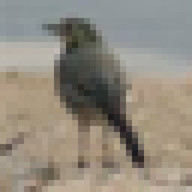
\includegraphics[width=1.25cm]{img/b_o0.png}};
\node[lab, anchor=north] at (0.75,-1.95) {画像 $\vec{x}$};
\node[sm, anchor=north, text=black!70] at (0.75,-2.33) {$3{\times}32{\times}32$ 個の数};
\draw[->] (1.45,-1.25) -- node[above, lab] {$+\sigma_{1}\vec{\varepsilon}$} (2.3,-1.25);
% the 34 blocks: resolution of the output 32, 16, 8 (height 1.5, 1.0, 0.6 cm)
\def\blk#1#2#3{% index, resolution, style
  \pgfmathsetmacro{\bx}{2.45+(#1-1)*0.17}
  \ifnum#2=32 \def\bh{1.5}\def\bc{-1.0}\fi
  \ifnum#2=16 \def\bh{1.0}\def\bc{-1.4}\fi
  \ifnum#2=8 \def\bh{0.6}\def\bc{-1.75}\fi
  \draw[#3] (\bx,\bc-\bh/2) rectangle ++(0.11,\bh);}
\foreach \i/\r in {1/32,2/32,3/32,4/32,5/32,6/16,8/16,9/16,10/16,11/8,12/8,13/8,14/8,15/8,16/8,17/8,18/8,19/8,20/8,21/8,22/8}
  {\blk{\i}{\r}{black, line width=0.45pt}}
\blk{7}{16}{navyc, line width=1.1pt}
\blk{23}{16}{redc, line width=1.1pt}
\foreach \i/\r in {24/16,25/16,26/16,27/16,28/16,29/32,30/32,31/32,32/32,33/32,34/32}
  {\blk{\i}{\r}{black!35, densely dashed, line width=0.4pt}}
\node[lab, anchor=south] at (5.31,-0.2) {U-Net(凍結)\ \ ブロックは34個};
\node[lab, text=navyc, anchor=south] at (3.53,-0.86) {$h$};
\node[lab, text=redc, anchor=south east] at (6.36,-0.86) {(ここで止める)A};
\node[sm, text=black!50, anchor=north] at (7.25,-2.0) {使わない};
\draw[decorate, decoration={brace, mirror, amplitude=3pt}] (2.45,-2.38) -- (6.30,-2.38);
\node[lab, anchor=north] at (4.38,-2.5) {ブロック1〜A ($p=23$ 個)};
\draw[->] (8.45,-0.75) -- (16.05,-0.75);
\node[lab, anchor=south] at (12.2,-0.7) {ブロック1〜Aのそれぞれから数を1つ\\(振幅 $a_{h}$)読み,縦に並べる};
\node[lab, anchor=north, text=black!70] at (12.2,-0.82) {1つの数の読み方は(b)};
% ---- the profile: p x 1, cells of 0.19 cm
\begin{scope}[shift={(16.15,-0.15)}]
  \foreach \k in {1,...,23} \draw[black, line width=0.4pt] (0,{-(\k-1)*0.19}) rectangle ++(0.3,-0.19);
  \draw[navyc, line width=1.1pt] (0,{-6*0.19}) rectangle ++(0.3,-0.19);
  \draw[redc, line width=1.1pt] (0,{-22*0.19}) rectangle ++(0.3,-0.19);
  \node[sm, anchor=west] at (0.33,-0.095) {$a_{1}$};
  \node[sm, anchor=west, text=navyc] at (0.33,{-6.5*0.19}) {$a_{h}$};
  \node[sm, anchor=west, text=redc] at (0.33,{-22.5*0.19}) {$a_{p}$(A)};
  \node[lab, anchor=south] at (0.15,0.02) {$\vec{a}(\vec{x})$};
  \node[sm, anchor=north] at (0.15,-4.43) {$p{\times}1$};
\end{scope}
% ================================================================ (b)
\begin{scope}[shift={(0,-0.2)}]
\node[ttl] at (0,-3.0) {\textbf{(b)}\ ブロック $h$(紺. 図では7番目)の出力から数を1つ読む(式~\eqref{eq:amp}の\cn{1}〜\cn{4})};
% stack of the C_h channel maps
\foreach \s in {4,3,2,1,0} \draw[black, line width=0.45pt, fill=white] ({0.25+0.1*\s},{-3.35-0.1*\s}) rectangle ++(1.25,-1.25);
\node[sm, anchor=north] at (1.15,-5.12) {$C_{h}=256$ 枚};
\node[sm, anchor=north] at (1.15,-5.45) {(チャネル $j$)};
\draw[->] (2.05,-4.15) -- node[above, sm] {$j$ 枚目} (2.65,-4.15);
% one channel: 16 x 16 values (cell 0.1 cm)
\begin{scope}[shift={(2.75,-3.35)}, x=0.1cm, y=0.1cm]
  \cellsraw
  \draw[black, line width=0.45pt] (0,0) rectangle (16,-16);
\end{scope}
\node[sm, anchor=north] at (3.55,-5.0) {$U_{h}=16{\times}16$ 個の値};
\node[sm, anchor=north] at (3.55,-5.33) {$f_{h,j,u}(\vec{x})$};
\draw[->] (4.45,-4.15) -- (6.15,-4.15);
\node[sm, anchor=south] at (5.3,-4.08) {\cn{1}\,平均を引く};
\node[sm, anchor=north] at (5.3,-4.22) {\cn{2}\,絶対値};
% |f - mean|: the largest one in red
\begin{scope}[shift={(6.25,-3.35)}, x=0.1cm, y=0.1cm]
  \cellsdev
  \draw[black, line width=0.45pt] (0,0) rectangle (16,-16);
  \draw[redc, line width=1.0pt] (\cellmaxcol,-\cellmaxrow) rectangle ++(1,-1);
\end{scope}
\node[sm, anchor=north] at (7.05,-5.0) {$|f_{h,j,u}(\vec{x})-\bar{f}_{h,j}(\vec{x})|$};
\node[sm, anchor=north, text=redc] at (7.05,-5.38) {最大のもの(赤)};
\draw[->] (7.95,-4.15) -- (9.15,-4.15);
\node[sm, anchor=south] at (8.55,-4.08) {\cn{3}\,最大の};
\node[sm, anchor=north] at (8.55,-4.22) {対数};
\draw[redc, line width=0.9pt] (9.25,-4.0) rectangle ++(0.3,-0.3);
\node[sm, anchor=north] at (9.4,-4.38) {数1つ};
\draw[->] (9.65,-4.15) -- (10.45,-4.15);
\node[sm, anchor=south] at (10.05,-4.08) {$j$ ごとに};
% the C_h numbers of block h
\foreach \k in {0,...,9} \draw[black, line width=0.4pt] ({10.55+0.22*\k},-4.04) rectangle ++(0.22,-0.22);
\node[sm] at (12.95,-4.15) {$\cdots$};
\foreach \k in {0,1} \draw[black, line width=0.4pt] ({13.2+0.22*\k},-4.04) rectangle ++(0.22,-0.22);
\draw[decorate, decoration={brace, mirror, amplitude=3pt}] (10.55,-4.38) -- (13.64,-4.38);
\node[sm, anchor=north] at (12.1,-4.5) {$C_{h}=256$ 個の数};
\draw[->] (13.75,-4.15) -- (14.55,-4.15);
\node[sm, anchor=south] at (14.15,-4.08) {\cn{4}\,平均};
\draw[navyc, line width=1.1pt] (14.65,-4.0) rectangle ++(0.3,-0.3);
\node[sm, anchor=north, text=navyc] at (14.8,-4.38) {$a_{h}(\vec{x})$};
\node[sm, anchor=north, text=navyc] at (14.8,-4.72) {数1つ};
\end{scope}
\draw[->, navyc, line width=0.7pt] (14.95,-4.15) .. controls (15.6,-3.9) and (15.5,-1.6) .. (16.1,-1.4);
\end{tikzpicture}

\caption{手順1：画像1枚から数を $p$ 個とる(CIFAR-10のモデル). (a) 34個のブロックを,出力の大きさ($32{\times}32$, $16{\times}16$, $8{\times}8$)に合わせた高さで描いた. 紺：ブロック $h$. 赤：ブロックA(23番目). その後の11個は計算しない. (b) 式~\eqref{eq:amp}の\cn{1}〜\cn{4}. 地図の濃淡は模式図である(濃いほど大きい).}
\label{fig:amp}
\end{figure}

\section{手順2：振幅が下がる向きを知る}
\label{sec:step2}
正方形の画像の向きの変え方は,そのままを除いて7つある(図~\ref{fig:orient}(a)). 画素を並べ替えるだけなので,画素の値の集まりは変わらない. この並べ替えを行列 $\Gm_{1},\dots,\Gm_{7}$ で書く. それでも見慣れない画像になり,振幅が下がる(図~\ref{fig:orient}(b)). 分布外の画像も下がる.

\begin{figure}[H]\centering
% f3_orient.tex -- Figure 3: the seven other orientations of the square, and what they do to the amplitudes (natural width about 17.2 cm).
%   (a) the eight orientations of one CIFAR-10-like image (bird.png of the slides): as it is (navy frame) and the seven G_k.
%   (b) a schematic of the per-block mean amplitudes (gen/mk_data.py, not data): ID (navy, band = +-1 SD), the seven re-oriented means
%       (grey), an OOD mean (red).  The measured shares are in the text (main resume, Table 7).
\begin{tikzpicture}[>={Stealth[length=1.8mm, width=1.4mm]}, line cap=round, line join=round, font=\footnotesize,
  lab/.style={inner sep=1pt, align=center, font=\footnotesize}, sm/.style={inner sep=1pt, align=center, font=\scriptsize},
  ttl/.style={anchor=west, inner sep=0pt, font=\small}]
% written by gen/mk_data.py: schematic per-block mean amplitudes (drawing coordinates, cm), p = 23
\def\profid{(8.350,-1.893) -- (8.716,-1.897) -- (9.082,-1.818) -- (9.448,-1.685) -- (9.814,-1.676) -- (10.180,-1.858) -- (10.545,-2.081) -- (10.911,-2.175) -- (11.277,-2.176) -- (11.643,-2.238) -- (12.009,-2.385) -- (12.375,-2.452) -- (12.741,-2.322) -- (13.107,-2.096) -- (13.473,-1.965) -- (13.839,-1.952) -- (14.205,-1.908) -- (14.570,-1.760) -- (14.936,-1.642) -- (15.302,-1.712) -- (15.668,-1.924) -- (16.034,-2.086) -- (16.400,-2.119)}
\def\profidhi{(8.350,-1.653) -- (8.716,-1.657) -- (9.082,-1.578) -- (9.448,-1.445) -- (9.814,-1.436) -- (10.180,-1.618) -- (10.545,-1.841) -- (10.911,-1.935) -- (11.277,-1.936) -- (11.643,-1.998) -- (12.009,-2.145) -- (12.375,-2.212) -- (12.741,-2.082) -- (13.107,-1.856) -- (13.473,-1.725) -- (13.839,-1.712) -- (14.205,-1.668) -- (14.570,-1.520) -- (14.936,-1.402) -- (15.302,-1.472) -- (15.668,-1.684) -- (16.034,-1.846) -- (16.400,-1.879)}
\def\profidlo{(8.350,-2.133) -- (8.716,-2.137) -- (9.082,-2.058) -- (9.448,-1.925) -- (9.814,-1.916) -- (10.180,-2.098) -- (10.545,-2.321) -- (10.911,-2.415) -- (11.277,-2.416) -- (11.643,-2.478) -- (12.009,-2.625) -- (12.375,-2.692) -- (12.741,-2.562) -- (13.107,-2.336) -- (13.473,-2.205) -- (13.839,-2.192) -- (14.205,-2.148) -- (14.570,-2.000) -- (14.936,-1.882) -- (15.302,-1.952) -- (15.668,-2.164) -- (16.034,-2.326) -- (16.400,-2.359)}
\def\profors{(8.350,-1.893) -- (8.716,-1.897) -- (9.082,-1.818) -- (9.448,-1.685) -- (9.814,-1.676) -- (10.180,-1.846) -- (10.545,-2.114) -- (10.911,-2.262) -- (11.277,-2.226) -- (11.643,-2.300) -- (12.009,-2.495) -- (12.375,-2.575) -- (12.741,-2.453) -- (13.107,-2.213) -- (13.473,-2.124) -- (13.839,-2.148) -- (14.205,-2.061) -- (14.570,-1.955) -- (14.936,-1.811) -- (15.302,-1.915) -- (15.668,-2.127) -- (16.034,-2.351) -- (16.400,-2.371) (8.350,-1.893) -- (8.716,-1.897) -- (9.082,-1.818) -- (9.448,-1.685) -- (9.814,-1.676) -- (10.180,-1.875) -- (10.545,-2.120) -- (10.911,-2.185) -- (11.277,-2.233) -- (11.643,-2.299) -- (12.009,-2.468) -- (12.375,-2.607) -- (12.741,-2.441) -- (13.107,-2.255) -- (13.473,-2.168) -- (13.839,-2.130) -- (14.205,-2.118) -- (14.570,-1.994) -- (14.936,-1.892) -- (15.302,-1.943) -- (15.668,-2.211) -- (16.034,-2.427) -- (16.400,-2.395) (8.350,-1.893) -- (8.716,-1.897) -- (9.082,-1.818) -- (9.448,-1.685) -- (9.814,-1.676) -- (10.180,-1.843) -- (10.545,-2.122) -- (10.911,-2.251) -- (11.277,-2.249) -- (11.643,-2.356) -- (12.009,-2.500) -- (12.375,-2.609) -- (12.741,-2.520) -- (13.107,-2.252) -- (13.473,-2.166) -- (13.839,-2.153) -- (14.205,-2.146) -- (14.570,-1.980) -- (14.936,-1.899) -- (15.302,-2.000) -- (15.668,-2.263) -- (16.034,-2.451) -- (16.400,-2.433) (8.350,-1.893) -- (8.716,-1.897) -- (9.082,-1.818) -- (9.448,-1.685) -- (9.814,-1.676) -- (10.180,-1.916) -- (10.545,-2.143) -- (10.911,-2.230) -- (11.277,-2.251) -- (11.643,-2.338) -- (12.009,-2.557) -- (12.375,-2.589) -- (12.741,-2.484) -- (13.107,-2.298) -- (13.473,-2.175) -- (13.839,-2.181) -- (14.205,-2.131) -- (14.570,-2.037) -- (14.936,-1.928) -- (15.302,-2.065) -- (15.668,-2.284) -- (16.034,-2.448) -- (16.400,-2.522) (8.350,-1.893) -- (8.716,-1.897) -- (9.082,-1.818) -- (9.448,-1.685) -- (9.814,-1.676) -- (10.180,-1.891) -- (10.545,-2.078) -- (10.911,-2.186) -- (11.277,-2.260) -- (11.643,-2.328) -- (12.009,-2.528) -- (12.375,-2.679) -- (12.741,-2.483) -- (13.107,-2.286) -- (13.473,-2.202) -- (13.839,-2.220) -- (14.205,-2.180) -- (14.570,-2.054) -- (14.936,-1.986) -- (15.302,-2.073) -- (15.668,-2.264) -- (16.034,-2.477) -- (16.400,-2.536) (8.350,-1.893) -- (8.716,-1.897) -- (9.082,-1.818) -- (9.448,-1.685) -- (9.814,-1.676) -- (10.180,-1.886) -- (10.545,-2.113) -- (10.911,-2.247) -- (11.277,-2.218) -- (11.643,-2.330) -- (12.009,-2.545) -- (12.375,-2.565) -- (12.741,-2.545) -- (13.107,-2.270) -- (13.473,-2.236) -- (13.839,-2.201) -- (14.205,-2.229) -- (14.570,-2.087) -- (14.936,-1.946) -- (15.302,-2.121) -- (15.668,-2.364) -- (16.034,-2.507) -- (16.400,-2.559) (8.350,-1.893) -- (8.716,-1.897) -- (9.082,-1.818) -- (9.448,-1.685) -- (9.814,-1.676) -- (10.180,-1.862) -- (10.545,-2.116) -- (10.911,-2.219) -- (11.277,-2.319) -- (11.643,-2.367) -- (12.009,-2.573) -- (12.375,-2.639) -- (12.741,-2.515) -- (13.107,-2.327) -- (13.473,-2.216) -- (13.839,-2.245) -- (14.205,-2.217) -- (14.570,-2.098) -- (14.936,-1.975) -- (15.302,-2.089) -- (15.668,-2.399) -- (16.034,-2.520) -- (16.400,-2.569)}
\def\profood{(8.350,-1.785) -- (8.716,-1.789) -- (9.082,-1.710) -- (9.448,-1.704) -- (9.814,-1.706) -- (10.180,-1.874) -- (10.545,-2.213) -- (10.911,-2.307) -- (11.277,-2.337) -- (11.643,-2.396) -- (12.009,-2.612) -- (12.375,-2.671) -- (12.741,-2.580) -- (13.107,-2.346) -- (13.473,-2.238) -- (13.839,-2.343) -- (14.205,-2.259) -- (14.570,-2.166) -- (14.936,-2.063) -- (15.302,-2.145) -- (15.668,-2.381) -- (16.034,-2.610) -- (16.400,-2.636)}
\def\profxA{16.400}\def\profyA{-2.119}\def\profyAor{-2.484}\def\profyAood{-2.636}
\def\profxone{8.350}

% ================================================================ (a)
\node[ttl] at (0,0.3) {\textbf{(a)}\ 向きの変え方は,そのままを除いて7つ};
\foreach \f/\x/\y/\t in {o0/0.7/-0.85/{}, vflip/2.35/-0.85/上下反転, hflip/4.0/-0.85/左右反転, r180/5.65/-0.85/180度回転,
                         r90/0.7/-2.75/90度回転, r270/2.35/-2.75/270度回転, tr/4.0/-2.75/{対角線で\\反転}, atr/5.65/-2.75/{もう1本の\\対角線で反転}}
  {\node[inner sep=0, draw=black!50, line width=0.4pt] at (\x,\y) {\includegraphics[width=1.15cm]{img/b_\f.png}};
   \node[sm, anchor=north] at (\x,{\y-0.64}) {\t};}
\draw[navyc, line width=1.3pt] (0.105,-0.255) rectangle (1.295,-1.445);
\node[sm, anchor=north, text=navyc] at (0.7,-1.49) {そのまま};
\node[sm, anchor=north west, align=left] at (0.0,-4.4) {そのまま以外の7つが $\mathbf{G}_{1}\vec{x},\dots,\mathbf{G}_{7}\vec{x}$(画素の並べ替え)};
% ================================================================ (b)
\draw[->, line width=0.9pt] (6.75,-1.8) -- (7.65,-1.8);
\node[sm, anchor=south] at (7.2,-1.75) {U-Netに};
\node[sm, anchor=north] at (7.2,-1.85) {通す};
\node[ttl] at (7.9,0.3) {\textbf{(b)}\ ブロックごとの振幅の平均(模式図)};
\draw[->, black!80] (8.05,-3.45) -- (16.95,-3.45);
\draw[->, black!80] (8.05,-3.45) -- (8.05,-0.3);
\node[lab, anchor=north] at (12.2,-3.5) {ブロック $h$};
\node[lab, anchor=west] at (8.15,-0.38) {振幅 $a_{h}$};
\node[sm, anchor=north] at (\profxone,-3.5) {1};
\node[sm, anchor=north, text=redc] at (\profxA,-3.5) {A};
\draw[black!45, densely dotted] (\profxA,-3.45) -- (\profxA,-0.6);
% ID band and mean
\draw[navyc!70, densely dotted, line width=0.5pt] \profidhi;
\draw[navyc!70, densely dotted, line width=0.5pt] \profidlo;
\draw[black!40, line width=0.45pt] \profors;
\draw[redc, line width=1.0pt] \profood;
\draw[navyc, line width=1.2pt] \profid;
\node[sm, text=navyc, anchor=south west, align=left] at (8.4,-1.2) {分布内の画像(そのまま). 点線：$\pm1$ 標準偏差};
\node[sm, text=black!60, anchor=north west] at (11.0,-3.0) {向きを変えた画像(7つの向き)};
\node[sm, text=redc, anchor=north west] at (8.65,-2.6) {分布外の画像};
\draw[->, line width=0.8pt] ({\profxA+0.25},\profyA) -- ({\profxA+0.25},\profyAood);
\node[sm, anchor=west] at ({\profxA+0.3},{(\profyA+\profyAood)/2}) {下がる};
\end{tikzpicture}

\caption{手順2の準備：向きを変えた分布内の画像. (a) 8つの向き. (b) ブロックごとの振幅の平均の模式図. 向きを変えた画像(灰)と分布外の画像(赤)は,分布内の画像(紺)より下がる.}
\label{fig:orient}
\end{figure}

CIFAR-10では,Aまでの23ブロックのうち,向きを変えると65\%,分布外の画像では70\%のブロックで,振幅の平均が分布内の平均より下がった(val2. 分布内の標準偏差の0.2倍以上低いブロックの割合. 分布外は集合ごとの値の平均. 本編の表7). そこで,分布外の画像を使わずに,分布内の画像 $\vx_{1},\dots,\vx_{n}$(val1. CIFAR-10では $n=\olNRefMax$)で振幅が下がる向きを求める. プロファイルの平均を
\begin{equation}
\vmu=\frac{1}{n}\sum_{i=1}^{n}\va(\vx_{i})
\label{eq:mu}
\end{equation}
共分散行列を $\Sm$($p\times p$),向きを変えたときの平均を
\begin{equation}
\vmu_{o}=\frac{1}{7n}\sum_{k=1}^{7}\sum_{i=1}^{n}\va(\Gm_{k}\vx_{i})
\label{eq:muo}
\end{equation}
とする. $\vmu-\vmu_{o}$ は $\vmu_{o}$ から $\vmu$ へ向かう矢印で,振幅が下がる向きの逆を指す(図~\ref{fig:space}の黒の矢印).

\section{手順3：基準点までの距離をスコアにする}
\label{sec:step3}
$\vmu$ を $\vmu-\vmu_{o}$ の向きへ $c$ 倍だけ動かした点を基準点とする($c=8$. 開発用の分割val2で決めた).
\begin{equation}
\vmu^{*}=\vmu+c(\vmu-\vmu_{o})
\label{eq:mustar}
\end{equation}
距離の重みの行列を
\begin{equation}
\Pm=(\Sm+\lambda\bar{s}\Id)^{-1}
\label{eq:prec}
\end{equation}
とし($\bar{s}$ は $\Sm$ の対角成分の平均, $\lambda=10^{-3}$),スコアを $\vmu^{*}$ までのマハラノビス距離の2乗にマイナスをつけたものとする.
\begin{equation}
s(\vx)=-\{\va(\vx)-\vmu^{*}\}^{\top}\Pm\{\va(\vx)-\vmu^{*}\}
\label{eq:score}
\end{equation}
形は $(1\times p)(p\times p)(p\times 1)$ で, $s(\vx)$ は数1つである(図~\ref{fig:shape}(a)).

\begin{figure}[H]\centering
% f4_space.tex -- Figure 4: the profile space, drawn to scale for CIFAR-10 (natural width about 17.3 cm).
%   Whitened coordinates: one unit = one ID standard deviation measured with P (P ~ S^-1), so the ordinary distance in the picture is the
%   Mahalanobis distance.  Horizontal axis: the direction of mu - mu_o; vertical: one of the other p - 1 = 22 directions.
%   mu = (0, 0), mu_o = (-Delta, 0), mu* = (c Delta, 0) with Delta = 1.768 and c = 8 (olx_info.json).  The clouds are schematic
%   (gen/mk_data.py).  Red dashed circles: equal score (circles about mu*).  Colours: navy = ID, grey = re-oriented, red = mu* and OOD.
\begin{tikzpicture}[>={Stealth[length=1.8mm, width=1.4mm]}, line cap=round, line join=round, font=\footnotesize,
  lab/.style={inner sep=1pt, align=center, font=\footnotesize}, sm/.style={inner sep=1pt, align=center, font=\scriptsize}]
% written by gen/mk_data.py: schematic clouds in whitened coordinates (unit = one ID standard deviation), Delta = 1.768
\def\iddots{1.141/-0.915, 0.793/-0.396, -0.460/0.787, 0.258/-0.211, -0.391/-0.483, 1.610/-0.506, 0.348/-0.784, 1.777/0.323, -2.663/0.210, -1.614/1.601, 0.070/-0.577, -0.432/-0.972, 0.960/-1.231, -0.113/-1.618, -0.096/-0.026, -0.013/-0.091, 1.323/0.224, 0.288/0.800, 1.522/-0.368, -0.714/0.926, -1.364/0.934, 1.369/0.839, 1.282/-2.040, -0.463/-0.773, 0.823/-0.255, 0.763/-0.393, 1.487/-1.352, 1.386/0.398, -0.270/0.410, 0.430/0.463, 0.877/-0.427, -0.372/-0.239, 1.049/-0.658, 0.223/-1.839, -0.944/-0.816, 0.348/0.524, -1.523/0.989, 2.220/-0.857, -1.523/1.908, -0.124/-0.016, -0.895/0.780, -1.154/-0.740, -0.883/-0.517}
\def\ordots{-1.181/-0.324, -2.756/0.911, 0.444/0.636, -3.820/-0.668, -1.408/0.078, -1.856/1.755, -0.855/0.710, -3.603/0.487, -2.943/1.209, -1.415/-1.033, -1.930/0.523, -0.329/-0.267, -2.925/-0.010, -2.026/0.355, -2.910/-0.731, -2.447/-0.342, -1.286/1.351, -3.754/-0.026, -1.556/0.315, -3.228/-0.173, -2.023/0.231, -2.999/-0.910, 0.621/0.860, -1.495/0.729, -2.527/0.524, -0.797/0.393, -0.870/0.235, -1.771/0.334, -2.710/-1.838, -3.078/-1.015, -1.412/0.120, -2.912/0.736, -2.381/2.031, -1.829/0.285, -2.386/0.150, -2.385/1.099, -1.830/0.783, -2.075/-0.558, -1.726/1.890, -2.952/-0.393, -1.908/-0.029, -2.152/-1.155, 0.660/-0.254, -2.828/0.498}
\def\mDelta{1.768}

\begin{scope}[shift={(3.75,0)}, x=0.78cm, y=0.78cm]
  \pgfmathsetmacro{\cD}{8*\mDelta}
  \draw[black!35, line width=0.4pt] (-4.6,-2.55) rectangle (15.3,2.55);
  \begin{scope}
    \clip (-4.6,-2.55) rectangle (15.3,2.55);
    \draw[black!25, line width=0.4pt] (-4.6,0) -- (15.3,0);
    \foreach \r in {3,6,...,18} \draw[redc!75, densely dashed, line width=0.5pt] (\cD,0) circle (\r);
    \foreach \a/\b in \ordots \fill[black!40] (\a,\b) circle (1.25pt);
    \foreach \a/\b in \iddots \fill[navyc] (\a,\b) circle (1.25pt);
  \end{scope}
  \draw[navyc, line width=0.5pt] (0,0) circle (1);
  \node[sm, text=navyc, anchor=north, fill=white, inner sep=0.5pt] at (0,-1.06) {1標準偏差};
  % means and the two arrows
  \fill[black!60] (-\mDelta,0) circle (2.2pt);
  \fill[navyc] (0,0) circle (2.2pt);
  \draw[->, line width=1.0pt] (-\mDelta+0.12,0) -- (-0.12,0);
  \node[lab, anchor=south, fill=white, inner sep=0.5pt] at (-0.88,0.16) {$\vec{\mu}-\vec{\mu}_{o}$};
  \node[lab, anchor=north, fill=white, inner sep=0.5pt] at (-\mDelta,-0.15) {$\vec{\mu}_{o}$};
  \node[lab, anchor=north, text=navyc, fill=white, inner sep=0.5pt] at (0.05,-0.15) {$\vec{\mu}$};
  \draw[->, redc, densely dashed, line width=1.0pt] (0.15,0) -- (\cD-0.2,0);
  \node[lab, text=redc, anchor=south, fill=white, inner sep=1pt] at (6.95,0.12) {$c(\vec{\mu}-\vec{\mu}_{o})$, \ $c=8$};
  \node[redc, font=\Large, inner sep=0] at (\cD,0) {$\star$};
  \node[lab, text=redc, anchor=south, fill=white, inner sep=1pt] at (\cD,0.3) {$\vec{\mu}^{*}$(基準点)};
  % the two test images
  \draw[navyc, line width=0.9pt] (0.5,0.8) circle (3.2pt);
  \draw[navyc, line width=0.4pt] (0.62,0.95) -- (1.45,1.75);
  \node[sm, text=navyc, anchor=west, fill=white, inner sep=1pt] at (1.45,1.82) {分布内のテスト画像};
  \fill[redc] (-3.3,-0.8) circle (3.0pt);
  \draw[redc, line width=0.4pt] (-3.3,-0.95) -- (-3.2,-1.35);
  \node[sm, text=redc, anchor=north, fill=white, inner sep=1pt, align=center] at (-3.1,-1.35) {分布外のテスト画像\\(振幅が下がった)};
  % names of the clouds
  \node[sm, text=black!65, anchor=north west, fill=white, inner sep=1pt] at (-4.5,2.45) {向きを変えた画像};
  \node[sm, text=navyc, anchor=west, fill=white, inner sep=1pt] at (1.9,-1.55) {分布内の画像};
  \node[sm, text=redc, anchor=north, fill=white, inner sep=1pt, align=center] at (7.0,-1.4) {スコアが等しい線\\($\vec{\mu}^{*}$ を中心とする円)};
  % axes
  \node[sm, anchor=west, align=left] at (15.35,0) {$\vec{\mu}-\vec{\mu}_{o}$\\の向き};
  \node[sm, anchor=south west] at (-4.6,2.58) {縦：ほかの向き(実際は $p-1=22$ 個). 縮尺：分布内の標準偏差をそろえた座標(ここでの距離がマハラノビス距離)};
  \draw[<->, line width=0.6pt] (-2.0,-3.0) -- (10.5,-3.0);
  \node[sm, anchor=east] at (-2.1,-3.0) {スコアが低い};
  \node[sm, anchor=west] at (10.6,-3.0) {スコアが高い};
\end{scope}
\end{tikzpicture}

\caption{手順3：プロファイルの空間(CIFAR-10の $\Delta=\olDeltaCten$, $c=8$ で縮尺どおり). 横：$\vmu-\vmu_{o}$ の向き. 縦：ほかの向きの1つ. 点は模式図(紺：分布内,灰：向きを変えた画像). $\vmu^{*}$ は $\vmu$ から $\vmu-\vmu_{o}$ の8倍だけ右にある. 赤の破線：スコアが等しい線.}
\label{fig:space}
\end{figure}

図~\ref{fig:space}は,分布内のばらつきが1になるように軸をとった図で,図の中のふつうの距離がマハラノビス距離である. $\vmu^{*}$ が遠いので,分布内の画像の付近では,スコアが等しい線(円)はほぼ縦になる. スコアはおもに横の位置で決まり,左(振幅が下がる側)へ外れた画像ほど低い.

\begin{figure}[H]\centering
% f5_shape.tex -- Figure 5: the shapes in eq. (8) and eq. (13) for p = 23 (CIFAR-10); one cell = one number (natural width about 15 cm).
%   (a) s(x) = - (1 x p)(p x p)(p x 1) = 1 x 1.  (b) l(x) = (1 x p)(p x 1) = 1 x 1, the inner product of v and P u.
\begin{tikzpicture}[line cap=round, line join=round, font=\footnotesize,
  sm/.style={inner sep=1pt, align=center, font=\scriptsize}, lab/.style={inner sep=1pt, align=center, font=\footnotesize},
  ttl/.style={anchor=west, inner sep=0pt, font=\small}]
\def\cs{0.1}
\def\rowv#1#2{% left x, centre y: a 1 x 23 row
  \draw[black, line width=0.5pt] (#1,#2+\cs/2) rectangle ++(23*\cs,-\cs);
  \foreach \k in {1,...,22} \draw[black!45, line width=0.2pt] ({#1+\k*\cs},#2+\cs/2) -- ++(0,-\cs);}
\def\colv#1#2{% centre x, top y: a 23 x 1 column
  \draw[black, line width=0.5pt] (#1-\cs/2,#2) rectangle ++(\cs,-23*\cs);
  \foreach \k in {1,...,22} \draw[black!45, line width=0.2pt] (#1-\cs/2,{#2-\k*\cs}) -- ++(\cs,0);}
% ---------------------------------------------------------------- (a) the score
\node[ttl] at (0,1.75) {\textbf{(a)}\ スコア $s(\vec{x})$[式~\eqref{eq:score}]};
\node[lab, anchor=east] at (1.25,0) {$s(\vec{x})=-$};
\rowv{1.35}{0}
\node[sm, anchor=south] at (2.5,0.1) {$\{\vec{a}(\vec{x})-\vec{\mu}^{*}\}^{\top}$};
\node[sm, anchor=north] at (2.5,-0.1) {$1{\times}p$};
\draw[black, line width=0.5pt] (3.85,1.15) rectangle ++(2.3,-2.3);
\foreach \k in {1,...,22} {\draw[black!15, line width=0.15pt] ({3.85+\k*\cs},1.15) -- ++(0,-2.3); \draw[black!15, line width=0.15pt] (3.85,{1.15-\k*\cs}) -- ++(2.3,0);}
\node[lab, anchor=south] at (5.0,1.18) {$\mathbf{P}$};
\node[sm, anchor=north] at (5.0,-1.2) {$p{\times}p$};
\colv{6.4}{1.15}
\node[sm, anchor=south] at (6.4,1.18) {$\vec{a}(\vec{x})-\vec{\mu}^{*}$};
\node[sm, anchor=north] at (6.4,-1.2) {$p{\times}1$};
\node[lab] at (6.85,0) {$=$};
\draw[redc, line width=0.9pt] (7.1,\cs/2) rectangle ++(\cs,-\cs);
\node[sm, anchor=south, text=redc] at (7.15,0.12) {数1つ};
\node[sm, anchor=north, text=redc] at (7.15,-0.12) {$1{\times}1$};
% ---------------------------------------------------------------- (b) the inner product term
\begin{scope}[shift={(9.3,0)}]
\node[ttl] at (0,1.75) {\textbf{(b)}\ 内積の項 $\ell(\vec{x})$[式~\eqref{eq:ell}]};
\node[lab, anchor=east] at (1.25,0) {$\ell(\vec{x})=$};
\rowv{1.35}{0}
\node[sm, anchor=south] at (2.5,0.1) {$\vec{v}^{\top}=(\vec{\mu}-\vec{\mu}_{o})^{\top}$};
\node[sm, anchor=north] at (2.5,-0.1) {$1{\times}p$};
\colv{3.95}{1.15}
\node[sm, anchor=south] at (3.95,1.18) {$\mathbf{P}\vec{u}$};
\node[sm, anchor=north] at (3.95,-1.2) {$p{\times}1$};
\node[lab] at (4.4,0) {$=$};
\draw[redc, line width=0.9pt] (4.65,\cs/2) rectangle ++(\cs,-\cs);
\node[sm, anchor=south, text=redc] at (4.7,0.12) {数1つ};
\node[sm, anchor=north, text=redc] at (4.7,-0.12) {$1{\times}1$};
\node[sm, anchor=west, align=left] at (5.05,-0.85) {横の並び $\times$ 縦の並び\\$=$ 内積(数1つ)};
\end{scope}
\end{tikzpicture}

\caption{形の確認($p=23$. 1マスが数1つ). (a) 式~\eqref{eq:score}. (b) 式~\eqref{eq:ell}：$\vv^{\top}$(横)と $\Pm\vu$(縦)の積,つまり内積. どちらも結果は $1\times 1$ の行列,つまり数1つ(スカラー)である.}
\label{fig:shape}
\end{figure}

\section{スコアを2つの項に分ける}
\label{sec:terms}
$\vu=\va(\vx)-\vmu$(テスト画像の,分布内の平均からのずれ), $\vv=\vmu-\vmu_{o}$ とおく. どちらも $p\times 1$ である. 式~\eqref{eq:mustar}から
\begin{equation}
\begin{split}
\va(\vx)-\vmu^{*}
&=\va(\vx)-\vmu-c(\vmu-\vmu_{o})\\
&=\vu-c\vv
\end{split}
\label{eq:shift}
\end{equation}
である. これを式~\eqref{eq:score}に入れて展開する.
\begin{equation}
\begin{split}
s(\vx)
&=-(\vu-c\vv)^{\top}\Pm(\vu-c\vv)\\
&=-\vu^{\top}\Pm\vu+c\,\vu^{\top}\Pm\vv+c\,\vv^{\top}\Pm\vu-c^{2}\vv^{\top}\Pm\vv\\
&=-\vu^{\top}\Pm\vu+2c\,\vv^{\top}\Pm\vu-c^{2}\vv^{\top}\Pm\vv
\end{split}
\label{eq:expand0}
\end{equation}
2行目から3行目では, $\vu^{\top}\Pm\vv$ が $1\times 1$ で転置しても変わらないことと, $\Pm$ が対称($\Pm^{\top}=\Pm$)であることを使った.
\begin{equation}
\begin{split}
\vu^{\top}\Pm\vv
&=(\vu^{\top}\Pm\vv)^{\top}\\
&=\vv^{\top}\Pm^{\top}\vu\\
&=\vv^{\top}\Pm\vu
\end{split}
\label{eq:sym}
\end{equation}
3つの項に名前をつける.
\begin{equation}
\begin{split}
d^{2}(\vx)
&=\vu^{\top}\Pm\vu\\
&=\{\va(\vx)-\vmu\}^{\top}\Pm\{\va(\vx)-\vmu\}
\end{split}
\label{eq:dsq}
\end{equation}
\begin{equation}
\begin{split}
\ell(\vx)
&=\vv^{\top}\Pm\vu\\
&=(\vmu-\vmu_{o})^{\top}\Pm\{\va(\vx)-\vmu\}
\end{split}
\label{eq:ell}
\end{equation}
\begin{equation}
\begin{split}
\Delta^{2}
&=\vv^{\top}\Pm\vv\\
&=(\vmu-\vmu_{o})^{\top}\Pm(\vmu-\vmu_{o})
\end{split}
\label{eq:delta}
\end{equation}
とおくと,式~\eqref{eq:expand0}は
\begin{equation}
s(\vx)=-d^{2}(\vx)+2c\,\ell(\vx)-c^{2}\Delta^{2}
\label{eq:expand}
\end{equation}
となる. 3つとも $(1\times p)(p\times p)(p\times 1)$ の形で,数1つである(図~\ref{fig:shape}).

\begin{figure}[H]\centering
% f6_terms.tex -- Figure 6: the two terms of eq. (15) in the same whitened coordinates as Figure 4 (natural width about 17.3 cm).
%   (a) d^2: equal on circles about mu (navy dashed); grows in every direction.
%   (b) l: equal on straight lines perpendicular to mu - mu_o; l is the position along that direction times Delta (l = Delta * horizontal
%       coordinate), so it is ONE number, read off a number line.  ID: mean 0, standard deviation about Delta; re-oriented: mean -Delta^2.
%   Same schematic clouds and test images as Figure 4; Delta = 1.768 (CIFAR-10).
\begin{tikzpicture}[>={Stealth[length=1.8mm, width=1.4mm]}, line cap=round, line join=round, font=\footnotesize,
  lab/.style={inner sep=1pt, align=center, font=\footnotesize}, sm/.style={inner sep=1pt, align=center, font=\scriptsize},
  ttl/.style={anchor=west, inner sep=0pt, font=\small}]
% written by gen/mk_data.py: schematic clouds in whitened coordinates (unit = one ID standard deviation), Delta = 1.768
\def\iddots{1.141/-0.915, 0.793/-0.396, -0.460/0.787, 0.258/-0.211, -0.391/-0.483, 1.610/-0.506, 0.348/-0.784, 1.777/0.323, -2.663/0.210, -1.614/1.601, 0.070/-0.577, -0.432/-0.972, 0.960/-1.231, -0.113/-1.618, -0.096/-0.026, -0.013/-0.091, 1.323/0.224, 0.288/0.800, 1.522/-0.368, -0.714/0.926, -1.364/0.934, 1.369/0.839, 1.282/-2.040, -0.463/-0.773, 0.823/-0.255, 0.763/-0.393, 1.487/-1.352, 1.386/0.398, -0.270/0.410, 0.430/0.463, 0.877/-0.427, -0.372/-0.239, 1.049/-0.658, 0.223/-1.839, -0.944/-0.816, 0.348/0.524, -1.523/0.989, 2.220/-0.857, -1.523/1.908, -0.124/-0.016, -0.895/0.780, -1.154/-0.740, -0.883/-0.517}
\def\ordots{-1.181/-0.324, -2.756/0.911, 0.444/0.636, -3.820/-0.668, -1.408/0.078, -1.856/1.755, -0.855/0.710, -3.603/0.487, -2.943/1.209, -1.415/-1.033, -1.930/0.523, -0.329/-0.267, -2.925/-0.010, -2.026/0.355, -2.910/-0.731, -2.447/-0.342, -1.286/1.351, -3.754/-0.026, -1.556/0.315, -3.228/-0.173, -2.023/0.231, -2.999/-0.910, 0.621/0.860, -1.495/0.729, -2.527/0.524, -0.797/0.393, -0.870/0.235, -1.771/0.334, -2.710/-1.838, -3.078/-1.015, -1.412/0.120, -2.912/0.736, -2.381/2.031, -1.829/0.285, -2.386/0.150, -2.385/1.099, -1.830/0.783, -2.075/-0.558, -1.726/1.890, -2.952/-0.393, -1.908/-0.029, -2.152/-1.155, 0.660/-0.254, -2.828/0.498}
\def\mDelta{1.768}

\def\plane{% frame, clouds and the two means (whitened units)
  \draw[black!35, line width=0.4pt] (-4.4,-2.35) rectangle (3.0,2.35);
  \begin{scope}
    \clip (-4.4,-2.35) rectangle (3.0,2.35);
    \foreach \a/\b in \ordots \fill[black!40] (\a,\b) circle (1.15pt);
    \foreach \a/\b in \iddots \fill[navyc] (\a,\b) circle (1.15pt);
  \end{scope}
  \fill[black!60] (-\mDelta,0) circle (2.1pt);
  \fill[navyc] (0,0) circle (2.1pt);
  \node[lab, anchor=north, fill=white, inner sep=0.5pt] at (-\mDelta,-0.15) {$\vec{\mu}_{o}$};
  \node[lab, anchor=north, text=navyc, fill=white, inner sep=0.5pt] at (0.05,-0.15) {$\vec{\mu}$};
  \draw[navyc, line width=0.9pt] (0.5,0.8) circle (3.0pt);
  \fill[redc] (-3.3,-0.8) circle (2.8pt);}
% ================================================================ (a)
\node[ttl] at (0,2.45) {\textbf{(a)}\ $d^{2}$：$\vec{\mu}$ からの距離の2乗};
\begin{scope}[shift={(3.7,0)}, x=0.8cm, y=0.8cm]
  \begin{scope}
    \clip (-4.4,-2.35) rectangle (3.0,2.35);
    \foreach \r in {1,2,3,4} \draw[navyc, densely dashed, line width=0.55pt] (0,0) circle (\r);
  \end{scope}
  \plane
  \node[sm, text=navyc, anchor=north, fill=white, inner sep=1pt, align=center] at (-0.7,-2.42) {$d^{2}$ が等しい線：$\vec{\mu}$ を中心とする円\\どの向きへ外れても $d^{2}$ は大きくなる};
\end{scope}
% ================================================================ (b)
\node[ttl] at (8.3,2.45) {\textbf{(b)}\ $\ell$：$\vec{\mu}-\vec{\mu}_{o}$ の向きの位置(数1つ)};
\begin{scope}[shift={(11.9,0)}, x=0.8cm, y=0.8cm]
  \begin{scope}
    \clip (-4.4,-2.35) rectangle (3.0,2.35);
    \foreach \x in {-4,-3,...,2} \draw[black!55, densely dashed, line width=0.5pt] (\x,-2.35) -- (\x,2.35);
  \end{scope}
  \plane
  \draw[->, line width=1.0pt] (-\mDelta+0.12,0) -- (-0.12,0);
  \node[sm, anchor=south, fill=white, inner sep=0.5pt] at (-0.88,0.14) {$\vec{\mu}-\vec{\mu}_{o}$};
  \node[sm, anchor=south west, fill=white, inner sep=1pt, align=left] at (-4.35,1.45) {$\ell$ が等しい線：\\$\vec{\mu}-\vec{\mu}_{o}$ に垂直な直線};
  % the number line of l (l = Delta * horizontal coordinate)
  \def\ny{-4.75}
  \draw[->, line width=0.7pt] (-4.4,\ny) -- (3.15,\ny);
  \node[lab, anchor=west] at (3.2,\ny) {$\ell$};
  \draw[black!60, line width=0.5pt, domain=-4.4:3.0, samples=60] plot (\x,{\ny+1.1*exp(-0.5*((\x+\mDelta)/0.93)^2)});
  \draw[navyc, line width=0.8pt, domain=-3.6:3.0, samples=60] plot (\x,{\ny+1.1*exp(-0.5*(\x)^2)});
  \draw[line width=0.6pt] (0,\ny-0.1) -- (0,\ny+0.1);
  \draw[line width=0.6pt] (-\mDelta,\ny-0.1) -- (-\mDelta,\ny+0.1);
  \node[sm, anchor=north] at (0,\ny-0.12) {$0$};
  \node[sm, anchor=north] at (-\mDelta,\ny-0.12) {$-\Delta^{2}$};
  \node[sm, text=navyc, anchor=south west, align=left] at (1.3,\ny+0.55) {分布内の画像\\平均 $0$,標準偏差 ${\approx}\,\Delta$};
  \node[sm, text=black!65, anchor=south east, align=right] at (-3.55,\ny+0.3) {向きを変えた画像\\平均 $-\Delta^{2}$};
  % the two test images dropped onto the line
  \draw[navyc, densely dotted, line width=0.6pt] (0.5,0.68) -- (0.5,\ny);
  \draw[redc, densely dotted, line width=0.6pt] (-3.3,-0.92) -- (-3.3,\ny);
  \fill[navyc] (0.5,\ny) circle (2.2pt);
  \fill[redc] (-3.3,\ny) circle (2.2pt);
\end{scope}
\node[lab, anchor=north west, align=left] at (0.3,-3.0) {(b)の $\ell$ は矢印(ベクトル)ではなく,\\数直線上の1点(スカラー)である.\\画像1枚に $\ell$ が1つ決まる\\(右下の数直線. 横の位置の $\Delta$ 倍).};
\end{tikzpicture}

\caption{式~\eqref{eq:expand}の2つの項(図~\ref{fig:space}と同じ座標と点). (a) $d^{2}$ は $\vmu$ を中心とする円の上で等しい. (b) $\ell$ は $\vmu-\vmu_{o}$ に垂直な直線の上で等しく,横の位置の $\Delta$ 倍である. 下の数直線の山は,分布内(紺)と向きを変えた画像(灰)の $\ell$ の分布の模式図. 紺の丸と赤の点：図~\ref{fig:space}の2枚のテスト画像.}
\label{fig:terms}
\end{figure}

\textbf{$d^{2}$(距離の項).} $\vmu$ を中心とする円の上で等しく,どの向きへ外れても大きくなる(図~\ref{fig:terms}(a)).

\textbf{$\ell$(内積の項).} $\vv$ と $\Pm\vu$ の内積で,数1つである(図~\ref{fig:shape}(b)). 図~\ref{fig:terms}(b)では横の位置の $\Delta$ 倍で, $\vmu-\vmu_{o}$ に垂直な直線の上で等しい. 分布内の画像では平均が0,標準偏差がほぼ $\Delta$ で,向きを変えた画像では平均が $-\Delta^{2}$ である. $2c=16$ がかかるので,スコアはおもに $\ell$ で決まる(図~\ref{fig:space}で等しい線がほぼ縦になる理由).

\textbf{$\Delta^{2}$.} 画像によらない定数で,画像の順位を変えない. CIFAR-10では $\Delta=\olDeltaCten$ である. 向きを変えてもプロファイルが動かないデータでは $\Delta$ が小さく, $\ell$ の幅も小さいので,内積の項は自動的に軽くなる(5つのモデルで $\Delta=\olDeltaMin$〜$\olDeltaMax$).

\section{まとめ：何をいつ計算するか}
表~\ref{tab:summary}のとおりである. 勾配による学習,追加のネットワーク,人手のラベル,分布外の画像は使わない.

\begin{table}[H]\centering\footnotesize\setlength{\tabcolsep}{6pt}\renewcommand{\arraystretch}{1.15}
\caption{用意するものと計算(右の列はCIFAR-10).}
\label{tab:summary}
\begin{tabular}{@{}p{18mm}p{92mm}p{38mm}@{}}\toprule
 & すること & CIFAR-10\\\midrule
用意する & 学習済みの拡散モデル(凍結)と,分布内の画像 $n$ 枚(val1) & $n=\olNRefMax$\\
事前に1回 & $n$ 枚を8つの向きでブロックAまで通す($8n$ 回の順伝播) & 16{,}000回\\
 & $\vmu$, $\Sm$, $\vmu_{o}$ から $\vmu^{*}$ と $\Pm$ を作る[式~\eqref{eq:mustar},~\eqref{eq:prec}] & \\
保存する & $\vmu^{*}$($p$ 個)と $\Pm$($p\times p$ 個)の数 & $23+529=552$ 個\\
テスト時 & ブロックAで止める順伝播1回 & 全体の\olFwdAShare\%の時間\\
 & 式~\eqref{eq:score}の計算1つ & \\\bottomrule
\end{tabular}
\end{table}

\end{document}
